\documentclass[12pt]{book}
\usepackage[top=1in, bottom=1in, left=1in, right=1in]{geometry}
\usepackage{amsmath}
\usepackage{tikz}
\usetikzlibrary[topaths]
\newcount\mycount
\usepackage{amssymb,latexsym}
%Loads these packages for math symbols.  
\usepackage{amsxtra}
%Loads extra accent symbols.
\usepackage{amsthm}
%Let you use the nice Theorem and Definition Environments.
\usepackage{graphicx}
%Lets you put graphics into your document.  I won't go into that here.
\usepackage{setspace}
%This is George Greenwade's package.  You can set spacing to be one-half or double using the following commands right here in the preamble:
\onehalfspacing
%\doublespacing would use double-spacing.
%\usepackage{hyperref}  %This allows you to make hyperlinks in your pdf and also within the document itself. We do not need this now but it could be useful later.
\usepackage{wasysym} %You can make smiley faces with this package. There are other symbols, too.  Google it.  Again, we likely will not use this.
\usepackage{verbatim} %This allows you to include LaTeX commands in your document (as text) that do not execute.  I use this to show you the LaTeX to type.
\usepackage{arcs}%You only need this if you are creating notation for arcs in geometry.  See Section 6.10
\usepackage{accents}
%What follows are called "Proclamations."  They are displayed text environments.
\theoremstyle{definition}
%This sets the style for proclamations.  The options are plain, definition, and remark.  You can try all three to see what they do.  "definition" does not put things in italics
%Since I do not like my theorems in italics, I use "definition."
%The following set up your declarations. For example, the first one writes "Definition" and the section number after you begin a definition. This helps with automatic numbering.

\usepackage{hyperref}
\hypersetup{
    colorlinks=true,
    linkcolor=black,
    filecolor=magenta,      
    urlcolor=cyan,
    pdftitle={Overleaf Example},
    pdfpagemode=FullScreen,
    }

\urlstyle{same}
%-----------------------------------------------------------------------------%
\newtheorem{definition}{Definition}[chapter]
\newtheorem{example}{Example}[chapter]
\newtheorem{theorem}{Theorem}[chapter]
\newtheorem{proposition}{Proposition}[section]
\newtheorem*{fact}{Fact}
\newtheorem{remark}{Remark}
\newtheorem{corollary}{Corollary}[section]
\newtheorem{lemma}{Lemma}[section]

% I do not want my facts numbered, so notice what I used.

%Next you can have some defintions, or shortcuts you use often.  Youwill come up with these for things you find yourself typing a lot.
\newcommand{\df}{\displaystyle \frac} 
\newcommand{\dlim}{\displaystyle \lim}
\newcommand{\dint}{\displaystyle \int}
\newcommand{\ra}{\rangle}
\newcommand{\la}{\langle}

\newcommand{\inner}[2]{{\langle #1,#2\rangle}}

\newcommand{\x}{\mathbf{x}}
\newcommand{\xt}{\mathbf{x}^{\mathsf{T}}}
\newcommand{\T}{{\mathsf{T}}}

\newcommand{\abf}{\mathbf{a}}
\newcommand{\abft}{\mathbf{a}^{\mathsf{T}}}
\newcommand{\R}{\mathbb{R}}
\newcommand{\C}{\mathbb{C}}
\newcommand{\E}{\mathrm{e}}
\newcommand{\F}{\mathbb{F}}
\newcommand{\X}{\mathbf{X}}
\newcommand{\Y}{\mathbf{Y}}

\newcommand{\f}{\mathbf{f}}
\newcommand{\U}{\mathbf{u}}
\newcommand{\D}{\mathrm{d}}
\newcommand{\M}{\mathcal{M}}
\newcommand{\LL}{\mathcal{L}}
\newcommand{\nullspace}{\mathrm{null}}
\newcommand{\range}{\mathrm{range}}
%%Operation
\newcommand{\Sum}[2]{{\sum_{#1}^{#2}}}
\newcommand{\Union}[2]{{\bigcup_{#1}^{#2}}}
\newcommand{\Intersection}[2]{{\bigcap_{#1}^{#2}}}
%You can use these so that you can type fractions or limits, and integrals within a line of text, and have it appear still in displaystyle. This is because I do not like the look of these inline.

\newcommand{\pd}[1]{\frac{\partial}{\partial #1}}
%The actual document starts now.

%-----------------------------------------------------------------------------%

\begin{document}

\title{Stochastic Mathematics in Finance}
\author{Nanyi, UIBE}
\maketitle % This actually puts the title, author, and date in.

%$$
%\begin{tikzpicture}[transform shape]
%  %the multiplication with floats is not possible. Thus I split the loop in two.
%  \foreach \number in {1,...,8}{
%      % Computer angle:
%        \mycount=\number
%        \advance\mycount by -1
%  \multiply\mycount by 45
%        \advance\mycount by 0
%      \node[draw,circle,inner sep=0.25cm] (N-\number) at (\the\mycount:5.4cm) {};
%    }
%  \foreach \number in {9,...,16}{
%      % Computer angle:
%        \mycount=\number
%        \advance\mycount by -1
%  \multiply\mycount by 45
%        \advance\mycount by 22.5
%      \node[draw,circle,inner sep=0.25cm] (N-\number) at (\the\mycount:5.4cm) {};
%    }
%  \foreach \number in {1,...,15}{
%        \mycount=\number
%        \advance\mycount by 1
%  \foreach \numbera in {\the\mycount,...,16}{
%    \path (N-\number) edge[->,bend right=3] (N-\numbera)  edge[<-,bend
%      left=3] (N-\numbera);
%  }
%}
%\end{tikzpicture}
%$$



%\begin{figure}[tp]
%	\begin{center}
%		\makeatletter
%		\def\@captype{figure}
%		\makeatother
%		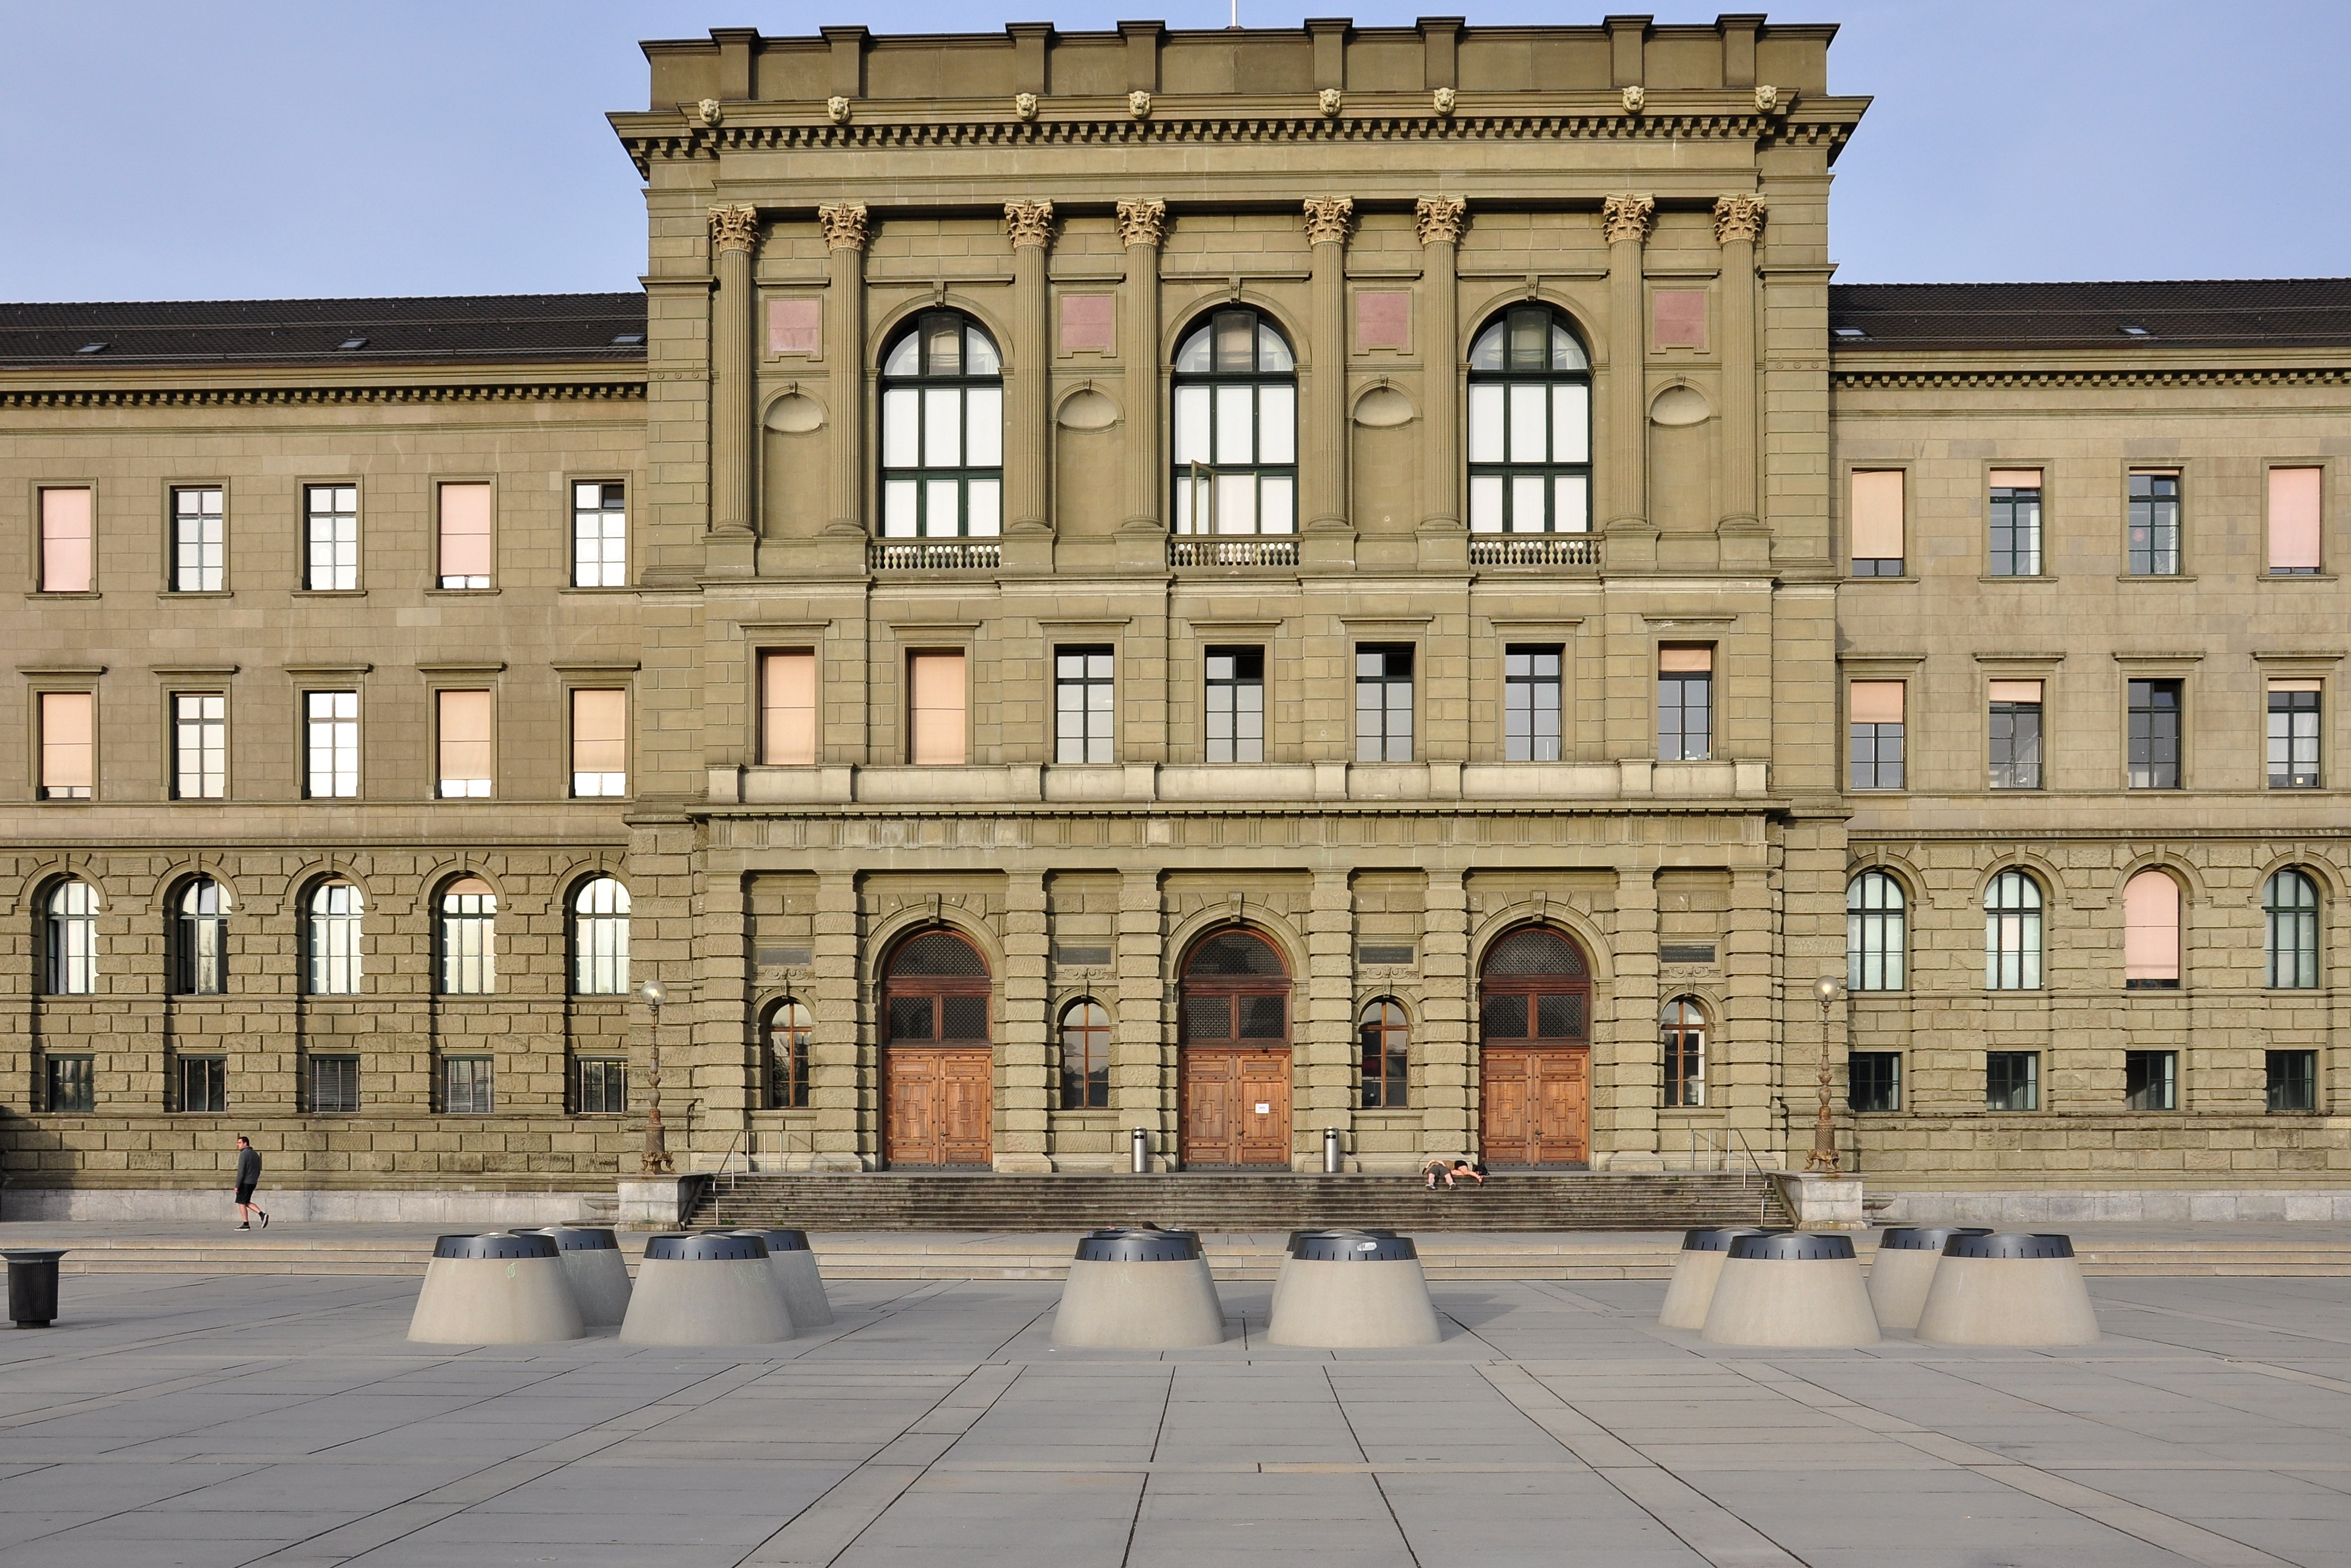
\includegraphics[scale=0.5]{figure/ETH.jpeg}
%		\caption{ETH zurich.} 
%	\end{center}
%\end{figure}

\tableofcontents
\clearpage
\addcontentsline{toc}{chapter}{Foreword}
{\huge {\bf Foreword}}
\mainmatter
%-----------------------------------------------------------------------------%

\chapter{Set Theory}

\section{Zermelo Fraenkel set theory}









\section{Logit gate}


\begin{definition}[Family] \ \\
Suppose $\Gamma$ is an index set, then a family $\{e_k\}_{k\in \Gamma}$ in a set $V$ is a function from $\Gamma$ to $V$.
$$
e : \Gamma \to V,\ k\mapsto e_k.
$$
\end{definition}

\begin{definition}[Union, Intersection, Complement] \ \\
 Suppose $A_k \subset \X$. Then the union of $A_k$ is defined by 
 $$
 \Union{k\in\Gamma}{} A_k := \{ x: \exists k_0 \in \Gamma, x\in A_{k_0}\}
 $$
 $$
 \Intersection{k\in\Gamma}{} A_k := \{ x: \forall k \in \Gamma, x\in A_{k}\}
 $$
 $$
 A^c := \{x: \notin A\}
 $$
 $$
 A \backslash B := \{x: x\in A,\ x \notin B \}
 $$
\end{definition}

\begin{definition}[Map] \ \\
Suppose $X$ and $Y$ are sets. A map $f$ from $X$ to $Y$ is a rule, which can be written by
$$
f: X \to Y,\ x \mapsto f(x),
$$
where $x \in X$ and $f(x) \in Y$.
\end{definition}

\begin{definition}[injection, bijection, surjection] \ \\
Suppose $f$ is a map from $X$ to $Y$. Then $f$ is an injection if for all 
$$
f(x_1) = f(x_2) \implies x_1=x_2.
$$
And $f$ is call a bijection if 
$$
\mathrm{range} f = Y.
$$
\end{definition}


\begin{definition}
	
\end{definition}





\begin{definition}[null space and range] \ \\
\end{definition}








\begin{theorem}[De moivre] \ \\
$$
(\Union{k\in\Gamma}{} A_k)^c =  \Intersection{k\in\Gamma}{} A_k^c
$$
\end{theorem}

\begin{definition}[Collection of set] \ \\
The set $\mathcal F$ whose elements are subsets of $X$ is called a collection of set on $X$.
\end{definition}

\begin{definition} Suppose $\mathcal F$ is a collection of set on $X$. Then 
	\begin{itemize}
		\item $\mathcal F$
	\end{itemize}
\end{definition}


\section{Binary Structure}
\begin{definition}[Binary operation] \ \\
A binary operation on a nonempty set $V$ is a map from $V \times V$ to $V$. In this case, the turple $(V,*)$ is called a binary structure.

\end{definition}

\begin{definition}[Semi-group] \ \\
A binary sturcture $(V,*)$ is called a semi-group if the operation $*$ is commutative. More precisely, $\forall a,b,c \in V$, we have
$$
a*(b*c) = (a*b)*c.
$$
In this case, the order of operation does not matter.
\end{definition}

\begin{definition}[Identity] \ \\
Suppose $(V,*)$ is a semi-group, then $e \in V$ is called an identity of $(V,*)$ if 
$$
e*a = a*e = a
$$
holds for all $a\in V$.
\end{definition}

\begin{definition}[Monoid] \ \\
A semigroup that has an indentity is called a monoid.
\end{definition}

\begin{theorem}
The identity on a monoid is unique.
\end{theorem}
\begin{proof}
Suppose $e,\tilde e$ are identities of a monoid $(S,*)$, then
$$
e = \tilde e *e = e*\tilde e= \tilde e.
$$	
\end{proof}


\begin{definition}[Inverse]
Suppose $(V,*)$ is a monoid. For all $a \in V$, if there exists (another) element $\tilde a\in V$ such that 
$$
a*\tilde a = \tilde a *a =e,
$$
then we say $\tilde a $ is the inverse of $a$.
\end{definition}

\begin{definition}[Group]
A monoid $(V,*)$ is said to be  a group if for all $a \in V$, there exists an inverse of $a$.
\end{definition}

\begin{theorem}
Operation inverse is unique.	
\end{theorem}

\begin{definition}[Abelian Group]
A group $(V,*)$ is Abelian if $\forall a,b \in V$,
$$
a*b=b*a.
$$
	
\end{definition}


\begin{example}[+ in python]
Let $V$ denote the class, list, in python. Then $(V,+)$ is a monoid.  
\end{example}
\begin{proof}
	Suppose $l_1,l_2 \in V$, then
$$
l_1 = [a_1,\cdots,a_n],
$$
$$
l_2 = [b_1,\cdots,b_m].
$$
And
$$
l_1 + l_2 = [a_1,\cdots,a_n,b_1,\cdots,b_m].
$$
Note that the identity is $[]$.
\end{proof}

\begin{remark}\
\begin{itemize}
	\item (character,+) is a monoid.
	\item (list,+) is a monoid.
	\item (float,+) is a Abelian group.
	\item (integer,+) is a Abelian group.
\end{itemize}
\end{remark}























\chapter{Banach Spaces}
We begin this chapter with a quick review of the essentials of metric spaces. Then we extend our results on measurable functions and integration to complex-valued functions. After that, we rapidly review the framework of vector spaces, which allows us to consider natural collections of measurable functions that are closed under addition and scalar multiplication.

Normed vector spaces and Banach spaces, which are introduced in the third section of this chapter, play a hugely important role in modern analysis. Most interest focuses on linear maps on these vector spaces. Key results about linear maps that we develop in this chapter include the Hahn-Banach Theorem, the Open Mapping Theorem, the Closed Graph Theorem, and the Principle of Uniform Boundedness.
\newpage
\section{Metric Space}
\begin{definition}[Metric Space] \ \\
A metric on a nonempty set $V$ is a function $d:V\times V \to [0,\infty)$ such that
\begin{itemize}
	\item $d(f,f)=0$ for all $f\in V$;
	\item $d(f,g)=0$ implies $f=g$;
	\item $d(f,g)=d(g,f$ for all $f,g \in V$;
	\item $d(f,h)\leq d(f,g)+d(g,h)$ for all $f,g,h \in V$. 
\end{itemize}
A metric space is a pair $(V,d)$, where $V$ is a nonempty set and $d$ is a metric on $V$.
\end{definition}

\begin{example}[Distance on $\R^n$] \ \\
Suppose $T$ is a positive self-adjoint operator. That is for all $f \in V$, 
$$
\inner{Tv}{v} = \inner{v}{T^* v} = \inner{v}{Tv}>0.
$$
Then we can define a distance on $\R^n$ by:
$$
d(x,y)^2 = \inner{x-y}{T(x-y)}=(x-y)^\prime \M(T) (x-y).
$$
\end{example}
\begin{example}[Minkowski Distance] \ \\ 
Suppose $X_1,\cdots,X_n$ is a random sample, where $X_1 = \begin{bmatrix}
	X_{11} \\
	X_{12} \\
	\vdots \\
	X_{1n}
\end{bmatrix}$ with mean $\mu$ and covariance matrix $\Sigma$. If $X_i$ are uncorrelated and $\x,\mathbf{y}\in \R^p$, then the distance between $\x$ and $\mathbf{y}$ is given by
$$
d^2(\x,\mathbf{y}) = (\x-\mathbf{y})^\prime \begin{bmatrix}
	\sigma_{11}^{-1} & & & \\
	 & \sigma_{22}^{-1} & & \\
	 & & \ddots & \\
	 & & & \sigma_{pp}^{-1}
\end{bmatrix} (\x-\mathbf{y}).
$$
\end{example}
However, if $X_i$ are correlated, we need to translate them into uncorrelated components and then use the above procedure to define the distance. To be specific, the real spectrum theorem yields that
$$
\Sigma = P\Lambda P^\prime , where \ \Lambda  = diag(\lambda_1,\cdots,\lambda_p).
$$
Thus the distance of $\x$ and $\mathbf{y}$ is defined by
\begin{eqnarray*}
d^2(\x,\mathbf{y}) & = &d^2(P^\prime(\x-\mu),P^\prime (\x-\mathbf{y})) \\
&=& (\x-\mathbf{y})^\prime P \Lambda^{-1}P^\prime(\x-\mathbf{y}) \\
&=& (\x-\mathbf{y})^\prime \Sigma^{-1} (\x - \mathbf{y})
\end{eqnarray*}











\begin{definition}[Open ball] \ \\
Suppose $(V,d)$ is a metric space, $f \in V$, and $r >0$.
\begin{itemize}
	\item The open ball centered at $f$ with radius $r$ is denoted by $B(f,r)$ and id defined by
	$$
	B(f,r) = \{g\in V: d(f,g) < r\}.
	$$
	\item The closed ball centered at $f$ with radius $r$ is denoted by $\overline{B}(f,r)$ and is defined by
	$$
	\overline{B}(f,r) = \{g\in V: d(f,g) \leq r\}.
	$$
\end{itemize}
\end{definition}

\begin{definition}[Open subset] \ \\
A subset $G$ of a metric space $V$ is called open if for all $f\in G$, there exists $r >0$ such that $B(f,r)\subset G$.
\end{definition}

\begin{definition}[Open subset] \ \\
A subset $F$ of a metric space $V$ is called close if $V\backslash F$ is open.
\end{definition}

\begin{definition}[closure] \ \\
Suppose $V$ is a metric space and $E\subset V$. Then the closure of $E$, denoted $\backslash E$, is defined by
$$
\overline{E} = \{g \in V: B(g,\varepsilon)\cap E \neq \emptyset,  \forall \varepsilon > 0\}
$$
\end{definition}

\begin{definition}[Limits in V]
Suppose $V$ is a metric space, $f_1,f_2,\cdots$ is a sequence in $V$, and $f\in V$. Then
	$$
\lim_{k \to \infty}f_k =f \ \text{means} \ \lim_{k \to \infty}d(f_k,f)=0
	$$
\end{definition}

\begin{theorem}[closure] \ \\
Suppose $V$ is a metric space and $E \subset V$. Then
\begin{itemize}
	\item $\overline{E}=\{ \}$
\end{itemize}	
\end{theorem}








\chapter{$L^p$ Spaces}
Fix a measure space $(X, \mathcal{S}, \mu)$ and a positive number $p$. We begin this chapter by looking at the vector space of measurable functions $f: X \rightarrow \mathbf{F}$ such that
$$
\int|f|^p d \mu<\infty .
$$
Important results called Holder's inequality and Minkowski's inequality help us investigate this vector space. A useful class of Banach spaces appears when we identify functions that differ only on a set of measure 0 and require $p \geq 1$.
\newpage
Suppose $(\X,\mathcal{S},\mu)$ is measure space, $0<p<\infty$.
\begin{definition}
	
\end{definition}


\begin{theorem}
Suppose $\mathbb{S}=\{\varphi: \varphi \ \text{is simple and } \ \varphi \in L^1(\X,\mathcal S,\mu) \}$. Then $\mathbb{S}$ is dense in $L^1(\X,\mathcal S,\mu)\}$.
\end{theorem}


\chapter{Hilbert Spaces}

Normed vector spaces and Banach spaces, which were introduced in Chapter 1 , capture the notion of distance. In this chapter we introduce inner product spaces, which capture the notion of angle. The concept of orthogonality, which corresponds to right angles in the familiar context of $\mathbf{R}^2$ or $\mathbf{R}^3$, plays a particularly important role in inner product spaces.

Just as a Banach space is defined to be a normed vector space in which every Cauchy sequence converges, a Hilbert space is defined to be an inner product space that is a Banach space. Hilbert spaces are named in honor of David Hilbert (1862-1943), who helped develop parts of the theory in the early twentieth century.

In this chapter, we will see a clean description of the bounded linear functionals on a Hilbert space. We will also see that every Hilbert space has an orthonormal basis, which make Hilbert spaces look much like standard Euclidean spaces but with infinite sums replacing finite sums.

\newpage
\section{Inner product space}
\begin{definition}[Inner Product on a vector space] \ \\
An inner product is a function from $V \times V$ to $\F$ and has the following properties.
\begin{itemize}
	\item Positivity: $\inner{f}{f}\in[0,\infty)$ for all $f\in V$.
	\item Definiteness: $\inner{f}{f}=0$ implies $f=0$.
	\item Linearity at first slot:
	\begin{eqnarray*}
		\inner{f+g}{h}&=&\inner{f}{h}+\inner{g}{h} \\
		\inner{af}{h} &=& a\inner{f}{h}
	\end{eqnarray*}
	\item Conjugate symmetry:
	$$
	\inner{f}{g} = \overline{\inner{g}{h}}
	$$
\end{itemize}
$(V,\inner{}{})$ is called an inner product space.
\end{definition}

\begin{theorem}[Properties of inner product] \ 
	\begin{enumerate}
		\item $\inner{0}{g} = \inner{g}{0}=0$.
		\item $\inner{f}{g+h}=\inner{f}{g}+\inner{f}{h}$.
		\item $\inner{f}{ag}=\overline{a}\inner{f}{g}.$
	\end{enumerate}
\end{theorem}
Define $\Vert f\Vert = \sqrt{\inner{f}{f}}$. and we say two elements of an inner product space are called orthogonal if their inner product equals 0.
\begin{theorem}[Pythagorean Theorem/Cauchy-Schwarz/Triangle Inequality]\
\begin{enumerate}
	\item $\Vert f+g \Vert^2=\Vert f\Vert^2 + \Vert g \vert^2$ iff $\inner{f}{g}=0$.
	\item $|\inner{f}{g}|\leq \Vert f \Vert \Vert g \Vert$. 
	\item $|\Vert f+g \Vert |\leq \Vert f\Vert + \Vert g \Vert$.
	\item $\Vert f+g \Vert^2+\Vert f-g \Vert^2=2\Vert f\Vert^2 + 2\Vert g \Vert^2$.   
\end{enumerate}
\end{theorem}
A direact consequence is that $(V,\Vert \Vert)$ is a normed vector space. And the distance of two elements of $V$ is defined by $d(f,g)=\Vert f-g\Vert$. 

\begin{definition}[Distance from a point to a set] \ \\
Suppose $f\in V$ and $U \subset V$. Then the distance between $f$ and $U$ is defined by
$$
d(f,U) := \inf\{d(f,g): g\in U \}. 
$$
Note also that $d(f,U)=0$ if and only if $f\in \overline{U}$	.
\end{definition}
\begin{proof} Recall that $\overline U =\{f\in V: B(f,\varepsilon)\cap E \neq \emptyset \ \text{for all} \ \varepsilon >0.\}$
Then
\begin{eqnarray*}
	d(f,U)=0 &\implies & \forall \varepsilon >0 ,\exists g\in U, s.t. \Vert f-g\Vert < \varepsilon \\
	& \implies & \forall \varepsilon >0, B(f,\varepsilon)\cap E\neq \emptyset. \\
	& \implies & f \in \overline U.
\end{eqnarray*}
And the other direction trivivally holds. 
\end{proof}

\begin{example}
Suppose $T$ is a positive self-adjoint operator on $V=\R^n$, which implies the matrix of $T$ is symmetric and positive defined. Then $d(u,v)=\inner{Tu}{v}=\nu^T\M(T)u$ is a distance on $V$.	
\end{example}

\begin{definition}
A complete inner product space is called a Hilbert space.	
\end{definition}

\begin{theorem}[Distance to a closed convex set is attained in a Hilbert space] \ \\
Suppose $V$ is a Hilbert space, $U$ is a non-empty closed convex set in $V$. Then there exists a unique $g\in U$ such that 
$$
\Vert f-g \Vert = d(f,U)
$$
\end{theorem}
\begin{proof}
By defition, there exists $g_n$ such that 
$$
\lim_{n \to \infty} \Vert f-g_n \Vert= d(f,U)
$$
Then for all m,n, we have 
\begin{eqnarray*}
	\Vert g_m-g_n\Vert^2 &=& \Vert (f-g_n)-(f-g_m)\Vert^2 \\
	&=& 2\Vert f-g_n\Vert^2 + 2\Vert f-g_m\Vert^2 - \Vert 2f-g_m-g_n\Vert^2 \\
	&=& 2\Vert f-g_n\Vert^2 + 2\Vert f-g_m\Vert^2 - 4 \Vert f-(g_m+g_n)/2\Vert^2 \\
	&\leq &  2\Vert f-g_n\Vert^2 + 2\Vert f-g_m\Vert^2 - 4d(f,U). 
\end{eqnarray*}
This implies $g_n$ is a Cauchy sequence in $V$, and thus exists $g\in V$ such that 
$$
\lim_{n \to \infty}|\vert g_n -g\Vert| = 0,
$$
since $V$ is complete. Also note that $U$ is closed, we have $g\in U$. This implies $d(f-g)\geq d(f,U)$. On the other hand,
$$
d(f,g) \leq d(f,g_n)+d(g_n,g),
$$
where the right side converges to $d(f,U)$. As for the uniqueness,..
\end{proof}
\section{Orthogonality}
\begin{definition}[Orthogonal Projection] \ \\
Suppose $U$ is a non-empty closed convex subset of a Hilbert space $V$. Then orthogonal projection of $V$ onto $U$ is the function
$$
P_U: V \to U, \ f\mapsto g. 
$$
Where $g$ is the only point that satisfies $d(f,g)=d(f,U)$. Theorem 3.3 admits our definition makes sense.
\end{definition}
\begin{remark}\
\begin{itemize}
	\item $P_U(f)=f$ iff $f\in U$.
	\item $P_U \circ P_U$ = $P_U$.
	\item Suppose $W$ is closed subspace and $W \subset U$,then $P_W=P_W \circ P_U$.
\end{itemize}
\end{remark}

\begin{definition}[Orthogonal Complement]
Suppose $U$ is a subset of an inner product space. Then
$$
U^{\perp} := \{ h\in V:h \perp U\}
$$
Note that $h \perp U$ implies $f\perp g $ for all $g\in U$.
\end{definition}

\begin{theorem}
Suppose $U$ is a closed subspace(or complete subspace) of a Hilbert space $V$. Then \begin{enumerate}
	\item $f-P_Uf$ is orthogonal to all $g \in U$.
	\item If $h \in U$ and $f-h \in U^\perp$, then $h=P_Uf$
	\item $P_U: V \to U$ is a bounded linear map. 
	\item $\Vert P_Uf\Vert\leq \Vert f\Vert$.
\end{enumerate}	
\end{theorem}
\begin{proof}
Suppose $g\in U$ and $a=-t\inner{f-P_Uf}{g}$ where $t>0$. Then we have
\begin{eqnarray*}
	\Vert f-P_Uf\Vert^2 &\leq & \Vert f - P_Uf +a g\Vert^2 \\
	&=& \Vert f-P_Uf \Vert^2 + |a|^2\Vert g\Vert^2 + 2\mathrm{Re} \overline{a} \inner{f-P_Uf}{g}.
\end{eqnarray*}
The inequality implies 
$$
2|\inner{f-P_u}{g}|^2 \leq t |\inner{f-P_u}{g}|^2 \Vert g\Vert^2.
$$
Thus $\inner{f-P_Uf}{g}=0$. \\
(2) Suppose $g \in U$. Since $U$ is a vector space, $g-h \in U$ and $\inner{f-h}{g-h}=0$, thus the triangle inequality implies 
\begin{eqnarray*}
	\Vert f -h \Vert^2 &\leq&  \Vert f -h \Vert^2 + \Vert h-g \Vert^2 \\
	&=& \Vert f-g \Vert^2.
\end{eqnarray*}
The inequality suggests that $h$ is the closest point with respect to $f$ in $U$ and thus $h=P_uf$. \\
(3) Suppose $f_1,f_2 \in V$. Since
$$
\inner{f_1+f_2-P_Uf_1-P_Uf_2}{g}=0
$$ 
for all $g \in U$. Now (2) implies that $P_U(f_1+f_2)=P_Uf_1+P_Uf_2$. \\
(4) At last, suppose $f=P_Uf + h$.
$$
\inner{P_Uf}{h} = \inner{P_Uf}{f-P_Uf}=0,
$$
since $P_Uf\in U$ and $f-P_Uf \perp U$. Thus 
$$
\Vert f\Vert^2 = \Vert P_Uf \Vert^2 + \Vert h \Vert^2. 
$$
\end{proof}

\begin{theorem}[Properties of Orthogonal Complement] \
\begin{enumerate}
	\item $U^\perp$ is a subspace of $V$.
	\item $U \cap U^\perp \subset \{0\}$.
	\item $W \subset U \implies U^\perp \subset W^\perp$.
	\item $(\overline U)^\perp=U^\perp$.
	\item $U \subset (U^\perp)^\perp$.
\end{enumerate}
\end{theorem}
\begin{proof}

\end{proof}

\begin{theorem}[Orthogonal Decomposition] \ \\
Suppose $U$ is a closed subspace of a Hilbert space $V$(and thus complete). Then 
$$
V = U \oplus U^\perp.
$$
In other words, $f\in V$ can can be uniquely written in the form
$$
f = g + h, \ g \in U,\ h \in U^\perp. 
$$
\end{theorem}

\begin{theorem}[Range and Null space of Orthogonal projections] \ \\
Suppose $U$ is a closed subspace of a Hilbert space $V$. Then
\begin{itemize}
	\item $\mathrm{range}P_U=U$ and $\mathrm{P_U}=U^\perp$.
	\item $\mathrm{range}P_{U^\perp} $
\end{itemize}

\end{theorem}

\begin{theorem}[Riesz Reprentation Theorem I]\label{Riesz Reprentation Theorem}
Suppose $\varphi \in B(V,\F)$ where $V$ is a Hilbert space. Then there exists a unique $h \in V$ such that 
$$
\varphi(f) = \inner{f}{h}
$$
for all $f \in V$. Moreover, $\Vert \varphi \Vert = \Vert h \Vert$.
\end{theorem}

\begin{proof}
Since $\nullspace \varphi \subset \{h\}^\perp$, which implies ${h}\subset (\nullspace \varphi)^\perp$. Thus we begin our proof with $(\nullspace \varphi)^\perp$. First suppose $\varphi \neq 0$, we claim that $\nullspace \varphi$ is a closed subspace of $V$ and $\nullspace \varphi \neq V$ since $\varphi$ is continuous.
Thus there exists $g \in (\nullspace \varphi)^\perp$ with $\Vert g\Vert=1$. Let
$$
h = \overline{\varphi(g)}g. 
$$
with $\Vert h\Vert^2=\inner{h}{h}=|\varphi(g)|^2$. Thus 
$$
\varphi(h) = |\varphi(g)|^2 = \Vert h \Vert^2.
$$
Now suppose $f \in V$,
\begin{eqnarray*}
	\inner{f}{h} &=& \inner{f-\frac{\varphi(f)}{\Vert h\Vert^2}h}{h} + \inner{\frac{\varphi(f)}{\Vert h\Vert^2}h}{h} \\
	&=& \inner{\frac{\varphi(f)}{\Vert h\Vert^2}h}{h} \\
	&=& \varphi(f),
\end{eqnarray*}
where the equality holds because $f-\frac{\varphi(f)}{\Vert h\Vert^2}h \in \nullspace \varphi$. \par
We have now proved the existence of $h$. To prove the uniqueness, suppose $\tilde h\in V$ has the same property. Then 
$$
\inner{h-\tilde h}{h - \tilde h}=\inner{h-\tilde h}{h}-\inner{h-\tilde h}{h}=\varphi(h-\tilde h)-\varphi(h-\tilde h)=0,
$$
which implies that $h=\tilde h$, which proves the uniqueness. \par
The Cauchy-Schwarz inequality implies 
$$
|\varphi(f)| = |\inner{f}{h}| \leq \Vert f\Vert \Vert h\Vert,
$$
and hence $\Vert \varphi \Vert \leq\Vert h \Vert$. On the other hand, 
$$
\varphi(h)=\Vert h\Vert^2, 
$$
we also have $\Vert \varphi \Vert \geq \Vert h \Vert$.
\end{proof}


\begin{theorem}[Riesz Reprentation Theorem II]\label{Riesz Reprentation Theorem II}
Suppose $\varphi \in B(V,\F)$ where $V$ is a Hilbert space. Let 
$$
h = \Sum{k\in \Gamma}{} \overline{\varphi(e_k)}e_k.
$$
Then 
$$
\varphi(f) = \inner{f}{h}
$$
for all $f\in V$. Furthermore, $\Vert \varphi \Vert=(\Sum{k\in \Gamma}{}|\varphi(e_k)|^2  )^{\frac{1}{2}}$.
\end{theorem}
\begin{proof}
	
\end{proof}






\section{Orthonormal Bases} \ \\

\begin{definition}
	$\{e_k\}_{k \in \Gamma}$ is called an orthonormal family if 
$$
\inner{e_i}{e_j}=\delta_{ij}, i,j \in \Gamma.
$$
\end{definition}
\begin{definition}[Unordered sum] \ \\
	Suppose $\{f_k\}_{k \in \Gamma}$ is a family in a normed vector space $V$. The unordered sum $\sum_{k \in \Gamma}$ is called convergent if $\exists g \in V$, $\forall \varepsilon >0$, $\exists \Omega \subset \Gamma$, for all $\Omega \subset \Omega^\prime \subset \Gamma$, we have
	$$
	\Vert g - \sum_{k\in \Omega^\prime}f_k \Vert < \varepsilon
	$$
If this happens, we set $\sum_{s\in \Gamma}f_k = g$. Moreover, if $\forall N >0$, $\exists \Omega \subset \Gamma$, for all $\Omega \subset \Omega^\prime \subset \Gamma$, we have
$$
\Vert \sum_{k\in \Omega^\prime}f_k \Vert > N
$$
We we say $\sum_{s\in \Gamma}f_k$ 'converges' to infinity.
\end{definition}

\begin{example}[Unordered sum in $\R$]\ 
	\begin{enumerate}
		\item $\{a_k\}_{k \in \Gamma}$ where $a_k$ is nonnegative.
$$
\sum_{k \in \Gamma}a_k = \sup\{\sum_{k \in \Omega}a_k: \Omega \ \text{is a finite subset of} \ \Gamma \}.
$$
If $\sup\{\sum_{k \in \Omega}a_k: \Omega \ \text{is a finite subset of} \ \Gamma \} < \infty$, then $\{a_k\}_{k \in \Gamma}$ is called convergent.
		\item General case.
$$
\sum_{k \in \Gamma}a_k \ \text{converges} \ \iff \sum_{k \in \Gamma}|a_k| < \infty.
$$
	\end{enumerate}
\end{example}

\begin{theorem}
Suppose $V$ is a Hilbert space, then the inner product defined on $V$ and the unordered sum operation are commutitative if the unordered sum makes sense.
\end{theorem}








\begin{theorem}[Linear combination of an orthonormal family] \ \\
Suppose $\{e_k\}_{k \in \Gamma}$ is an orthonormal family in a Hilbert space $V$, and also suppose $\{a_k\}_{k \in \Gamma}$ is a family in $\F$. Then
\begin{itemize}
	\item $\sum_{k \in \Gamma}a_ke_k \ converges$ $\iff (\sum_{k \in \Gamma}|a_k|^2)^{\frac{1}{2}}<\infty$ 
	\item Furthermore, if $\sum_{k \in \Gamma}a_ke_k \ converges$, then $\Vert \sum_{k \in \Gamma}a_ke_k\Vert^2=\sum_{k \in \Gamma}|a_k|^2$.
\end{itemize} 
\end{theorem}
\begin{proof}
First suppose $\sum_{k \in \Gamma}a_ke_k=g$. Then for all $\varepsilon > 0$, there exists $\Omega$ such that for all $\Omega \subset \Omega^\prime\subset \Gamma$ holds
$$
\Vert g - \sum_{k\in \Omega^\prime}a_ke_k\Vert < \epsilon.
$$
This implies 
$$
\Vert g \Vert - \varepsilon < \Vert \sum_{k \in \Omega^\prime}a_ke_k\Vert < \Vert g\Vert + \epsilon.
$$
You should note that $\Vert \sum_{k \in \Omega^\prime}a_ke_k\Vert=(\sum_{k\in \Omega^\prime}|a_k^2|)^{\frac{1}{2}}$, since $\Omega^\prime$ is a finite set. This inquality now implies that $\sum_{k\in \Gamma}|a_k^2|$ is convergent to $\Vert g \Vert^2$, in other words,
$$
\Vert \sum_{k \in \Gamma} a_ke_k \Vert = \Vert g\Vert= (\sum_{k\in \Gamma}|a_k^2|)^\frac{1}{2}.
$$
To prove the other direction of (i), now suppose $\sum_{k\in \Gamma}|a_k^2|<\infty$. Define
$$
\sum_{\Gamma \backslash \Omega}|a_k|^2 := \sum_{k \in \Gamma}|a_k|^2 - \sum_{k \in \Omega}|a_k|^2, \ \text{where Omega is a finite set.}
$$
The definition above makes sense, as you should verify. By definition, there exists an incresing set $\Omega_1\subset \Omega_2 \subset \cdots,$ such that 
$$
\sum_{k \in \Gamma \backslash \Omega_m} |a_k|^2 < \frac{1}{m^2}.
$$
Set $g_m = \sum{j\in \Omega_m}a_je_j$, then
$$
\Vert g_n -g_m \Vert ^2 = \sum_{\Omega_n \backslash \Omega_m}|a_j|^2<\frac{1}{m^2}.(why?)
$$
This implies that $g_n$ is a Cauchy sequence in $V$ and thus converges to some element $g \in V$. To show that $\sum_{k \in \Gamma}a_ke_k=g$, suppose $\Omega_m \subset \Omega^\prime $.
\begin{eqnarray*}
	\Vert g - \sum_{k \in \Omega^\prime}a_ke_k\Vert &\leq& \Vert g-g_m\Vert + \Vert g_m-\sum_{j \in \Omega^\prime}a_je_j \Vert \\
	&\leq & \frac{1}{m} + \frac{1}{m}.
\end{eqnarray*}
\end{proof}

\begin{theorem}[Bassel's inequility] \ \\
Suppose $\{e_k\}_{k \in \Gamma}$ is an orthonormal family in an inner product space $V$ and $f \in V$. Then we have
$$
\sum_{k\in \Gamma}|\inner{f}{e_k}|^2 \leq \Vert f \Vert^2,
$$
and thus $ \sum_{k \in \Gamma} \inner{f}{e_k}e_k$ converges.
\end{theorem}
\begin{proof}
Decomposing $f$ as follows:
\begin{eqnarray*}
	f &=& \sum_{j \in \Omega}\inner{f}{e_j}e_j + (f-\sum_{j \in \Omega}\inner{f}{e_j}e_j),
\end{eqnarray*}
where  the first part in the right side is orthogonal to the second part, as you should verify.
Applying the Pythagorean Theorem to the equation above and we obtain
\begin{eqnarray*}
\Vert f\Vert^2 &=& \Vert\sum_{j \in \Omega}\inner{f}{e_j}e_j \Vert^2 + \Vert(f-\sum_{j \in \Omega}\inner{f}{e_j}e_j) \Vert^2 \\
&\geq& \sum_{k \in \Omega}|\inner{f}{e_k}|^2.
\end{eqnarray*}
Take supremum, and we have
$$
\Vert f \Vert ^2 \geq \sum_{k \in \Gamma}|\inner{f}{e_k}|^2.
$$
\end{proof}
Recall that we have already define the span of a family by
$$
\mathrm{span}\{e_k\}_{k \in \Gamma} := \{\sum_{k \in \Omega}a_ke_k: \{a_k\}_{k \in \Omega} \ \text{is a finite subfamily of} \ \F\}.
$$
And the closure of $\mathrm{span}\{e_k\}_{k \in \Gamma}$ is 
$$
\overline{\mathrm{span}\{e_k\}_{k \in \Gamma}}=\left\{ g \in V: \forall \varepsilon>0, B(g,r)\cap \mathrm{span}\{e_k\}_{k \in \Gamma} \neq \emptyset \right\}.
$$
\begin{theorem}[Closure of the span of an orthonormal family] \ \\
Suppose $\{e_k\}_{k \in \Gamma}$ is an orthonormal family in a Hilbert space $V$. Then 
$$
\overline{\mathrm{span}\{e_k\}_{k \in \Gamma}} = \left\{ \sum_{k \in \Gamma}a_ke_k: \{a_k\}_{k \in \Gamma} \ \text{is a family in} \ \F \ \text{and}\ \sum_{k \in \Gamma}|a_k|^2 < \infty. \right\}
$$
Moreover, for all $f \in \overline{\mathrm{span}\{e_k\}_{k \in \Gamma}} $
$$
f = \sum_{k \in \Gamma} \inner{f}{e_k}e_k.
$$	
\end{theorem}
\begin{proof}
Note that $\overline{\mathrm{span}\{e_k\}_{k \in \Gamma}}$ is a vector space, as you should verify.
The set in the right is well-defined since $\sum_{k \in \Gamma}|a_k|^2 < \infty$. We start our proof with $\left\{ \sum_{k \in \Gamma}a_ke_k:  \sum_{k \in \Gamma}|a_k|^2 < \infty. \right\} \subset \overline{\mathrm{span}\{e_k\}_{k \in \Gamma}}$. \par
First note that for all $g$ in the left set, assume $g=\sum_{k \in \Gamma}a_ke_k$, for all $\varepsilon>0$, there exists $\Omega \subset \Gamma$, such that 
$$ 
\sum_{\Gamma \backslash \Omega}|a_k|^2 < \varepsilon^2,
$$
which implies 
$$
\Vert \sum_{k \in \Gamma}a_ke_k -\sum_{k \in \Omega}a_ke_k \Vert=\sum_{\Gamma \backslash \Omega}|a_k|^2 < \varepsilon.
$$
In other words, 
$$
B(g,\varepsilon)\cap \overline{\mathrm{span}\{e_k\}_{k \in \Gamma}} \neq\emptyset,
$$
and thus $g \in \overline{\mathrm{span}\{e_k\}_{k \in \Gamma}}$. \par
To prove the other direction, suppose $f \in \overline{\mathrm{span}\{e_k\}_{k \in \Gamma}}$, and 
$$
g = \sum_{k \in \Gamma}\inner{f}{e_k}e_k.
$$
The Bassel's inequility now implies $g$ is in the set in the right part, next, by the inclusion we have just proved, $g\in \overline{\mathrm{span}\{e_k\}_{k \in \Gamma}}$ and thus $f-g \in \overline{\mathrm{span}\{e_k\}_{k \in \Gamma}}$.
Also,
\begin{eqnarray*}
	\inner{g}{e_j} &=& \inner{\sum_{k \in \Gamma}\inner{f}{e_k}e_k}{e_j} \\
	&=& \sum_{k \in \Gamma}\inner{f}{e_k}\inner{e_k}{e_j} \\
	&=& \inner{f}{e_j}.
\end{eqnarray*}
Hence 
$$
\inner{f-g}{e_k}=0, \ \forall k \in \Gamma.
$$
This implies that 
$$
g-f \in\left(\operatorname{span}\left\{e_j\right\}_{j \in \Gamma}\right)^{\perp}=\left(\overline{\operatorname{span}\left\{e_j\right\}_{j \in \Gamma}}\right)^{\perp}
$$
Since $$
\left(\operatorname{span}\left\{e_j\right\}_{j \in \Gamma}\right)^{\perp} \cap \left(\overline{\operatorname{span}\left\{e_j\right\}_{j \in \Gamma}}\right)^{\perp} = \{0\},
$$
we have $g=f$.
\end{proof}


\begin{definition}[Orthonormal Basis] \ \\
An orthonormal family $\{e_k\}_{k \in \Gamma}$ in a Hilbert space is called an orthonormal family of $V$ if
$$
\overline{\mathrm{span}\{e_k\}_{k \in \Gamma}}= V
$$
	
\end{definition}

\begin{theorem}[Parseval's identity]
Suppose $\{e_k\}_{k \in \Gamma}$ is an orthonormal basis in a Hilbert space $V$. For all $f,g\in V$, we have
\begin{itemize}
	\item $f=\sum_{k \in \Gamma}\inner{f}{e_k}e_k$
	\item $\inner{f}{g}$
	\item $\inner{f}{f}= \sum_{k \in \Gamma}|\inner{f}{e_k}|^2$
\end{itemize}
\end{theorem}

\begin{example}[]
For $k \in \mathbf{Z}$, suppose $e_k:(-\pi, \pi] \rightarrow \mathbf{R}$ is defined by
$$
e_k(t)= \begin{cases}\frac{1}{\sqrt{\pi}} \sin (k t) & \text { if } k>0, \\ 
\frac{1}{\sqrt{2 \pi}} & \text { if } k=0, \\ 
\frac{1}{\sqrt{\pi}} \cos (k t) & \text { if } k<0\end{cases}
$$
Then $\{e_k\}_{k \in Z}$ is an orthonormal basis of $L^2((-\pi,\pi])$.
\end{example}





\chapter{Measure Theory} 
A measure is a countably additive function from a $\sigma$-algebra to $[0, \infty] .$ In this chapter, we consider countably additive functions from a $\sigma$-algebra to either $\mathbf{R}$ or $\mathbf{C}$. The first section of this chapter shows that these functions, called real measures or complex measures, form an a Banach space with total variation norm.

The second section of this chapter focuses on decomposition theorems that help us understand real and complex measures. Radon-Nikodym theorem is derived and 
these results will lead to a proof that the dual space of $L^p(\mu)$ can be identified with $L^{p^{\prime}}(\mu)$.
\newpage
\section{Complex Measures}
Suppose $(\X,\mathcal S)$ is a measurable space.
\begin{definition} \ \\
\begin{itemize}
	\item A function $\nu:S \to F$ is called countably additive if \\
	$$
	\nu(\bigcup_{n=1}^\infty E_n) = \sum_{n=1}^{\infty} \nu(E_n).
	$$
	\item A real measure on $(\X,\mathcal S)$ is a countably addtive function: $\nu : \mathcal S \to \R$.
	\item A complex measure on $(\X,\mathcal S)$ is a countably addtive function: $\nu : \mathcal S \to \C$.
\end{itemize}	
\end{definition}

\begin{remark} \
\begin{enumerate}
  \item 	We use the terminology (positive) measure to reprensent the function that maps $ \mathcal S \to [0,\infty]$.
  \item A finite measure is a real measure.
  \item $\M_{\C}(\mathcal S):=\{\nu:\nu \ \text{is a complex measure on}\ (\X,\mathcal S) \}$
\end{enumerate}
\end{remark}

\begin{definition}[addition and scalar multiplication] \ \\
for all $E\in \mathcal S$ and $a \in \F$, define
\begin{itemize}
	\item $\nu+\mu: E \mapsto \nu(E)+\mu(E)$.
	\item $a\nu: E \mapsto$ $a\nu(E)$.
\end{itemize}
\end{definition}
\begin{theorem}
$\M_\F(\mathcal S)$	is a vector space over $\F$.
\end{theorem}


\begin{theorem}\
Suppose $\nu \in \M_{\C}(\mathcal S)$, then 
\begin{enumerate}
	\item $\nu(\emptyset)=0$.
	\item $\sum_{n=1}^{\infty}|\nu(E_k)| < \infty$ for all disjoint sequence $E_1,\cdots$ of $\mathcal S$.
\end{enumerate}
\end{theorem}
\begin{proof}
$$
\nu(\emptyset) = \nu(\Union{n=1}{\infty}\emptyset) = \Sum{n=1}{\infty}\nu(\emptyset).
$$
This implies $\nu(\emptyset)=0$. \par
On the other hand, suppose F=R, making the following decomposition, we obtain
$$
$$
\end{proof}

\begin{theorem}\ \\
Suppose $\mu$ is a measure on $(\X,\mathcal S)$ and $h \in \LL(\mu)$. Define $\nu:\mathcal S \to \F$ by 
$$
\nu(E) = \int_E h \D \mu
$$
Then $\nu \in \M_\C(\mathcal S)$.
\end{theorem}

\begin{remark} \ \\
The $\nu$ defined above is often denoted by $h\D\mu$.
\end{remark}

\begin{theorem}[Properties of complex measures]\
\begin{enumerate}
	\item $\nu(E\backslash D) = \nu(E)-\nu(D) \ for \ all\  D \subset E.$
	\item $\nu(D \cup E) = \nu(D) + \nu(E) - \nu(D\cap E)$.
	\item for increasing sequence $E_n$,
	$$\nu(\Union{n=1}{\infty}E_n)=\lim_{n \to \infty}\nu(E_n). $$
	\item for decreasing sequence $E_n$,
	$$\nu(\Intersection{n=1}{\infty}E_n)=\lim_{n \to \infty}\nu(E_n). $$
\end{enumerate}
\end{theorem}

\begin{definition}[] \ \\
Total variation measure of $\nu$ is the function $|\nu|: \mathcal S \to [0,\infty]$ defined by
$$
|\nu| = \sup\{\Sum{k=1}{n}|\nu(E_k)|: E_i \cap E_j =\emptyset, \ \Union{k=1}{n}E_k \subset E\}.
$$
\end{definition}

\begin{theorem}[Properties of total variation measure] \ 
\begin{itemize}
	\item $|\nu(E)| \leq |\nu|(E)$ for all $E \in \mathcal S$.
	\item $|\nu|(E) = \nu(E)$ if $\nu$ is a finite measure.
	\item $|\nu|(E) = 0$ iff $\forall A\in \mathcal S, \ \nu(A)=0$.
	\item Equivalent definition: $$|\nu|(E)=\sup\{|\nu(A)|+|\nu(B)|: A\cap B=\emptyset \ and \ A \cup B \subset E \}.$$
\end{itemize}
\end{theorem}

\begin{theorem}[] \ \\
Total variation measure is indeed a complex measure on $(\X,\mathcal S)$. To be specific,
$$\nu \in \M_\F(\mathcal S) \ \text{implies} \ |\nu| \ \text{is a measure}.$$
\end{theorem}

\begin{definition}[Total variation norm] \ \\
$$
\Vert \nu \Vert := |\nu|(\X)
$$
\end{definition}

\begin{theorem}\label{Banach_Measure} 
$(\M_\F(\mathcal S),\Vert\Vert)$ is a Banach space.	
\end{theorem}
We perform the following procedures to prove this theorem.

\begin{proof} \
\begin{enumerate}
	\item $\forall \nu \in \M_\F(\mathcal S)$,$\Vert \nu \Vert=|\nu|(\X) <  \infty$.
	\item $\Vert \Vert$ is a norm on $\M_\F(\mathcal S)$.
	\item $(\M_{\F}(\mathcal S),\Vert \Vert)$ is complete. 
\end{enumerate}
S1. First suppose $\F=\R$ and $| \nu|(\X)=\infty$. \\
Provided that $E_n$ is well-defined such that $|\nu|(E_n)=\infty$ and $|\nu(E_n)|\geq n$.
By definition, there exists $A \subset E_n$ such that
$$
|\nu(A)| \geq n+1 + |\nu(E_n)|
$$
$$
|\nu(E_n \backslash A)| = |\nu(E_n)-\nu(A)| \geq n+1
$$
$$
|\nu|(A) + |\nu|(E_n\backslash A) = \infty.
$$
Since $|\nu|$ is a measure, we conclude at least one of $\nu|(A)$ and $|\nu|(E_n\backslash A)$ equals $\infty$. Thus we take
$$
E_{n+1} = A  \ if \  |\nu|(A)=\infty, \ otherwise \ E_{n+1} = E_n \backslash A.
$$
The procedure above induces a decreasing squence $E_n$ with
$$
\nu(\Intersection{n=1}{\infty}E_n) = \lim_{n \to \infty}\nu(E_n).
$$
Where the left side is well-defined since $\nu$ is a complex measure, while the right side does not exists. This contradicts to our assumption of $|\nu|(X)=\infty$. \\
S2. The proof of 2 is lefted to the reader. \\
S3. Suppose $\nu_n$ is Cauchy sequence in $\M_\F \mathcal S$. For each $E\in \mathcal S$, we have
\begin{eqnarray*}
	|\nu_i(E)-\nu_j(E)| &=& |(\nu_i-\nu_j)(E)| \\
	&\leq & |\nu_i-\nu_j|(E) \\
	&\leq & \Vert \nu_i - \nu_j \Vert.
\end{eqnarray*}
Which implies $\nu_i(E)$ is a Cauchy sequence in $\F$. Thus we define $\\nu$ as follows:
$$
\nu: \mathcal{S} \to \F, \ E \mapsto \lim_{j \to \infty}\nu_j(E).
$$
We make the following claims:
\begin{enumerate}
	\item $\lim_{n\to \infty} \Vert \nu_n-\nu\Vert =0$.
	\item $\nu$ is complex measure.
\end{enumerate}
For one thing, suppose $E_1,\cdots,E_n$ are disjoints subsets of $\X$. $\forall \varepsilon >0,\exists m >0$, for all i, j $\geq$ m. We have
\begin{eqnarray*}
	\Sum{l=1}{n}|\nu-\nu_k|(E_l) &=& \lim_{j \to \infty}\Sum{l=1}{n}|\nu_j-\nu_k|(E_l)\\
	&<&\lim_{j\to \infty} \Vert \nu_j - \nu_k \Vert \\
	&\leq& \varepsilon.
\end{eqnarray*}
The definition of $|\nu-\nu_k|(\X)$ implies 
$$
|\nu-\nu_k|(\X) = \Vert \nu -\nu_k \Vert < \varepsilon. 
$$
On the other hand, also suppose that $E_n$ are disjoint subsets of $X$, considering that
\begin{eqnarray*}
|\nu(\Union{k=1}{\infty}E_k)-\Sum{k=1}{n-1}\nu(E_k)| &=& |\lim_{j \to \infty}\nu_j(\Union{k=1}{\infty}E_k)-\lim_{j \to \infty}(\Sum{k=1}{n-1}\nu_j(E_k))| \\
&=& \lim_{j \to \infty}\Sum{k=n}{\infty}|\nu_j(E_k)|  \\
&=& \lim_{j \to \infty}\Sum{k=n}{\infty}|(\nu_j-\nu_m)(E_k)+\nu_m(E_k)| \\
&\leq & \lim_{j \to \infty}\Sum{k=n}{\infty}|(\nu_j-\nu_m)|(E_k)+\Sum{k=n}{\infty}|\nu_m(E_k)| \\
&\leq & \lim_{j \to \infty} \Vert \nu_j - \nu_m \Vert + \Sum{k=n}{\infty}|\nu_m(E_k)|.
\end{eqnarray*}
Then, we choose .... This completes the prove of Theorem \ref{Banach_Measure}.












\end{proof}

\section{Decomposition Theorem}
\begin{theorem}[Hahn Decomposition Theorem]\label{Hahn} \ \\
Suppose $\nu \in \M_\F(\mathcal S)$. Then there exsits $A,B\in \mathcal S$ such that
\begin{itemize}
	\item $A\cup B=\X$ and $A \cap B =\emptyset$.
	\item $\nu(E) \geq 0$ for all $E \subset A$.
	\item $\nu(E) \leq 0$ for all $E \subset B$.
\end{itemize}
\begin{proof}
Suppose $a = \sup\{\nu(E):E\in \mathcal S\}$. By definition, we have the following inequality
$$
a\leq \Vert \nu \Vert < \infty.
$$
The sequence $E_n$ is chosen to such that 
$$
\nu(E_j) \geq a - \frac{1}{2^j}.
$$
We claim that 
$$
A = \Intersection{k=1}{\infty}\Union{j=k}{\infty	} E_j, \ B = X\backslash A.
$$
To illustrate why $A$ meets our needs, we will show by induction on $n$ if $n\geq k$ holds
$$
\nu(\Union{j=k}{n}\nu(E_k)) \geq a - \Sum{j=k}{n	}\frac{1}{2^j}.
$$
To get started with the induction, note that if $n=k$, the equation clearly holds.
Suppose $n \geq k$ hold, then
\begin{eqnarray*}
	\nu(\Union{j=k}{n+1}E_j) &=& \nu(\Union{j=k}{n}E_k)+\nu(E_{n+1}) - \nu(\Union{j=k}{n}E_k \backslash E_{n+1}) \\
	&\geq& a - \Sum{j=k}{n}\frac{1}{2^j}+a - \frac{1}{2^{n+1}}-a \\
	&=& a-\Sum{j=k}{n+1}\frac{1}{2^j}.
\end{eqnarray*}
The continuity of measure admits 
$$
\nu(\Union{j=k}{\infty}A_j) \geq a-\frac{1}{2^{k-1}}
$$
and 
$$
\nu(\Intersection{k=1}{\infty}\Union{j=k}{\infty	} E_j)=a,
$$
and hence for all $E\in \mathcal S$ 
$$
\nu(E \cap A) = \nu(A) - \nu(A\cap E^c) \geq 0.
$$
Since $(E\cap B)\cap A =\emptyset$, we have
$$
\nu(E \cap B) = \nu(A\cup E \cap B)-\nu(A) \leq 0.
$$
This completes the proof of Theorem \ref{Hahn}.
\end{proof}
\end{theorem}

\begin{definition}
Suppose $\nu \in \M_\F(\mathcal S)$. $\nu$ is called lives on a set $A$ if for all $E\in \mathcal S$, we have
$$
\nu(E) = \nu(E\cap A)
$$ 	
\end{definition}
\begin{remark}
$\nu$ lives on $A$ implies for all $E \in A^c$, $\nu(E)=0$.	
\end{remark}


\begin{definition}[Singular Measures] \ \\
Suppose $\nu,\mu \in \M_\F(\mathcal S)$. Then $\nu$ and $\mu$ are called singular with    respect to each other, denoted $\nu \perp \mu$ if $\nu$ and $\mu$ live on different set. More precisely, there exists $A,B\in \mathcal S$ such that   
\begin{itemize}
	\item $A\cup B=\X$ and $A\cap B= \emptyset$.
	\item $\nu(E)=\nu(E\cap A)$ and $\mu(E)=\mu(E\cap B)$
\end{itemize}
\end{definition}


\begin{theorem}[Jordan Decomposition Theorem]\label{Joran_Decomposition} \ \\
Suppose $\nu$ is a real measure on $(\X,\mathcal S)$. Then there exists unique finite measures $\nu^+$ and $\nu^-$ on $(\X,\mathcal S)$ such that 
$$
\nu = \nu^+ - \nu^- \ \text{and} \ \nu^+ \perp \nu^-.
$$
Moreover, $|\nu|= \nu^+ + \nu^-$.
\end{theorem}
\begin{proof}
Let $\X=A\cup B$ be the Hahn Decomposition of $\nu$. Define
$$
\nu^+: \mathcal S \to [0,\infty),\ E \mapsto \nu(E\cap A),
$$
and 
$$
\nu^-: \mathcal S \to [0,\infty), \ E \mapsto -\nu(E\cap B).
$$
The contably addivity of $\nu$ implies $\nu^+$ and $\nu^-$ are finite measures on $(\X,\mathcal S)$ with 
$$
\nu = \nu^+ - \nu^-, \nu^+ \perp \nu^-. (\nu^+ \ \text{lives on}\  A \ \text{while} \ \nu^- \ \text{lives on}\  B)
$$
Let us turn to the proof of $\nu = \nu^+ + \nu^-$. First note that $\nu^+ + \nu^- $ is indeed a measure.\\
On the one hand, 
\begin{eqnarray*}
|\nu(E\cap A)| + |\nu(E\cap B)| &=& (\nu^+ + \nu^-)(E\cap A) + (\nu^+ + \nu^-)(E \cap B) \\
&=& (\nu^+ + \nu^-)(E).
\end{eqnarray*}
Which implies $|\nu|(E) \geq (\nu^+ +\nu^-)(E)$. \\
On the other hand, Suppose $E_1, E_2$ are disjoint subsets in $E$.
\begin{eqnarray*}
	|\nu(E_1)| + |\nu(E_2)| &=& |(\nu^+ - \nu^-)(E_1)| + |(\nu^+ - \nu^-)(E_2)| \\
	&\leq &  (\nu^+ + \nu^ -)(E_1) + (\nu^+ + \nu^ -)(E_2) \\
	&\leq & (\nu^+ + \nu^ -)(E).
\end{eqnarray*}
Take supreme of both sides, we obtain $|\nu(E)|\leq (\nu^+ + \nu^ -)(E)$.
As for the uniqueness, note also that
$$
\nu^+ = \frac{|\nu|+\nu}{2}, \ \nu^- = \frac{|\nu|-\nu}{2}.
$$
Since $|\nu|$ and $\nu$ are well-defined, $\nu^+$ can be uniquely identified by $\nu$.  This completes the proof of Theorem \ref{Joran_Decomposition}.
\end{proof}

\begin{remark} $\nu^+(\nu^-)$ is called the positive(negative) part of $\nu$.
\end{remark}

\begin{definition}[Integration with respect to real measures]
Suppose $\nu \in \M_R(\mathcal S)$, then the integral of $f$ is defined by
$$
\int_\X f \D \nu := \int_\X f \D \nu^+ - \int_\X f \D \nu^-
$$
\end{definition}





\begin{definition}[Absolutely continuous; $\ll$]
Suppose $\nu \M_\F(\mathcal S)$ and $\mu$ is a measure. Then $\nu$ is called absolutely continuous with respect to $\mu$ denoted by $\nu \ll \mu$ if 
$$
\mu(E)=0 \implies \nu(E)=0. 
$$
\end{definition}
Note that $\{\nu \in \M_\F(\mathcal S): \nu \ll \mu\}$ is a subspace.

\begin{theorem}
Suppose $\nu \in \M_\F(\mathcal S)$, then
$$
\nu \ll \mu \ \text{and} \ \nu \perp \mu \ \text{implies} \ \nu=0. 
$$	
\end{theorem}
\begin{proof}
Since $nu$ and $\mu$ are singular, there exists disjoints subsets such that $X=A\cup B$ and for all $E\in \mathcal S$ 
\begin{eqnarray*}
	\nu(E) &=& \nu(E\cap A) \\
	\mu(E) &=& \mu(E\cap B) \\
	\mu(E\cap A) &=& \mu(E\cap A \cap B) = 0.
\end{eqnarray*}
Also note that $\nu$ is absolutely continuous with respect to $\mu$, and thus we have
$$
\nu(E) = \nu(E \cap A) =0.
$$
Or $\Vert \nu \Vert=0$.
\end{proof}









\begin{theorem}[Lebesgue Decomposition Theorem] \ \\
Suppose $\mu$ is a measure and $\nu \in \M_\F(\mathcal S)$. Then there exsits unique $\nu_a,\nu_b \in \M_\F(\mathcal S)$ such that $\nu=\nu_a+\nu_s$ and 
$$
\nu_a \ll \mu \ \text{and} \ \nu_s \perp \mu.
$$
\end{theorem}
\begin{proof}
Let 
$$
b = \sup \{ |\nu|(B): B\in \mathcal S, \ \mu(B) = 0\},
$$
and $B_k$ be such that 
$$
|\nu|(B_k)\geq b -\frac{1}{k} \ \text{and} \ \mu(B_k)=0,
$$
Taking $B$ as 
$$
B = \Union{k=1}{\infty}B_k.
$$
then $\mu(B)=0$ and $|\nu(B)|=b$. Let A = $X\backslash B$ and 
\begin{eqnarray*}
	\nu_a &:& \mathcal S \to \F, \ E\mapsto \nu(E\cap A) \\
	\nu_s &:& \mathcal S \to \F, \ E\mapsto \nu(E\cap B).
\end{eqnarray*}
Clear $\nu = \nu_a + \nu_s$. Note also that 
$$
\mu(E) = \mu(E\cap A) + \mu(E \cap B) = \mu(E \cap A),
$$
which implies $\mu$ and $\nu_s$ live on different sets and thus mutually singular.
At last, to prove $\nu_a \ll \mu$, first suppose $\mu(E)=0$.
$$
\nu_a(E) = \nu(E\cap A) = \nu(E\backslash B)
$$
Since $\mu(E)=0$, we have $\mu(B\cup E)=0$ and thus
$$
b\geq |\nu|(B\cup E) = |\nu|(B) + |\nu|(E\backslash B) = b + |\nu|(E\backslash B).
$$
This implies $|\nu|(E\backslash B)=0$, and hence $\nu(E\backslash B)=0$.
As for the uniqueness, suppose $\nu_1,\nu_2$ be another Lebesgue-Decompositon of $\nu$ with respect to $\mu$. Then $\nu_a + \nu_s = \nu_1 + \nu_2$ implies
$$
\nu_a - \nu_1 = \nu_s - \nu_2.
$$
The left part is absolutely continuous to $\mu$ while the right part is singuar to $\mu$. 
Hence we conclude $\nu_1=\nu_a$ and $\nu_2=\nu_S$.
\end{proof}







\begin{theorem}[Radon-Nikodym Theorem] \ \\
Suppose $\mu$ is a $\sigma$-finite measure on a measurable space $(\X,\mathcal S)$. Suppose $\nu$ is a complex measure $(\X,\mathcal S)$ such $\nu \ll \mu$. Then there exists $h \in \LL^1(\mu)$ such that $\D \nu = h\D \mu$.
\end{theorem}
\begin{proof} \ \\
Step 1. Suppose $\nu$ and $\mu$ are finite measures on $(\X,\mathcal S)$. \\
For all $f \in L^2(\nu+\mu)$, define $\varphi$ as 
$$
\varphi : L^2(\nu+\mu) \to \R, \ f \mapsto \int_\X f \D \nu.
$$ 
To see why our definition makes sense, note that 
$$
\int_\X |f| \D \nu \leq \int_\X |f| \D (\nu+\mu) \leq (\nu(\X)+\mu(\X))^{\frac{1}{2}}\Vert f\Vert_{L^2(\nu+\mu)}.
$$
This implies $f\in L^2(\nu)$ and $\Vert \varphi \Vert \leq (\nu(\X)+\mu(\X))^{\frac{1}{2}}$.
Since $\nu$ is a bounded linear functional on $f \in L^2(\nu+\mu)$. The Riesz Representation Theorem now implies that there exists unique $g \in L^2(\nu+\mu)$ such that 
$$
\int_\X f \D \nu = \int_\X fg \D (\nu+\mu).
$$
Equvalently,
$$
\int_\X f(1-g) \D \nu = \int_\X fg \D \mu.
$$
Suppose 
\begin{eqnarray*}
	E_1 &=& \{ x\in \X: g(x) \geq 1   \}\\
    E_0 &=& \{ x\in \X: g(x) < 0   \}.
\end{eqnarray*}
And 
\begin{eqnarray*}
	&f=\chi_{E_1} \implies \mu(E_1) = 0 \implies \nu(E_1)=0 \\
	&f= \chi_{E_0} \implies \mu(E_0) = 0 \implies \nu(E_0)=0.
\end{eqnarray*}
Thus we can define $g$ as a function with range [0,1), and we define $h:\X \to [0,\infty)$ by
$$
h(x) = \frac{g(x)}{1-g(x)}.
$$
Then suppose $E\in\mathcal S$, and let $f_k$ be
$$
f_k(x) = \frac{\chi_E(x)}{1-g(x)}I_{\frac{\chi_E(x)}{1-g(x)}<k}(x).
$$
Easy to verify that $f_k$ is an increasing function with
$$
\int_\X f_k(x)^2 \D (\nu+\mu) \leq k^2 (\nu(\X)+\mu(\X)).
$$
Thus $f_k \in L^2(\nu+\mu)$ and hence 
$$
\int_\X f_k(1-g) \D \nu = \int_\X f_kg\D \mu
$$
The Monotone Convergence Theorem now implies 
$$
\int_\X \chi_E \D \nu = \int_\X \chi_E h \D \mu.
$$
Step 2. Suppose $\nu$ is a measure while $\mu$ is a $\sigma$-finite measure. \\
Now relex the assumption on $\mu$ to the hypothesis that $\mu$ is a $\sigma$-finite measure.
Thus there exsits an increasing sequence sets $\X_1\subset\X_2 \subset \cdots$ such that $\Union{j=1}{\infty}\X_j=\X$ and $\mu(\X_j)<\infty$.
Let $\nu_k,\mu_k$ be the restriction of $\nu,\mu$ on $\X_k$. Since $\nu_k$ and $\mu_k$ are finite measures, step1 implies there exists $h_k \in L^1(\mu)$ such that $\D \nu_k = h_k \D\mu_k$. Next, for $j<k$ and for all $E \in \mathcal S$, we have
\begin{eqnarray*}
	\int_{E\cap\X_j}h_j \D \mu_j &=& \int_{E\cap \X_j}h_j \D \mu \\
	&=& \nu_j(E\cap \X_j) \\
	&=& \nu_k(E \cap \X_j) \\
	&=& \int_{E \cap \X_j}h_k \D \mu.
\end{eqnarray*}
This implies 
$$
\mu(\{x\in \X_k: h_j(x)\neq h_k(x)\})=0.
$$
We conclude there exists $h:\X \to [0,\infty)$ such that 
$$
\mu(\{x\in \X_k: h(x)\neq h_k(x)\})=0
$$
for all $k>0$. Suppose otherwise ...
$$
\nu(E\cap \X_k) = \int_{E\cap \X_k} h\D \mu
$$
Let $k \to \infty$, and complete the proof. \\
Step 3. Suppose $\nu$ is a real measure while $\mu$ is a $\sigma$-finite measure. \\
Note that $|\nu|+\nu$ and $|\nu|-\nu$ are finite measures. By the case proved last page, there exists $h_+, h_- \in L^1(\mu)$ such that 
$$
\D (|\nu|+\nu) = h_+ \D \mu,\ \D (|\nu|-\nu) = h_- \D \mu.
$$
and 
$$
\D \nu = \frac{h_+ + h_-}{2}\D \mu.
$$
\end{proof}





































\begin{remark}
The construction of $h$ shows that it is undistinguishable on a set of zero measure with respect $\mu$,
\end{remark}

\begin{theorem}
Suppose $\nu$ is a complex measure and $\mu,\lambda$ are $\sigma$-finite measures on a measurable space $(\X,\mathcal S)$, 
\begin{enumerate}
	\item If $\nu \ll \mu$, then $g \in L^1(\X,\nu)$ implies $g\frac{\D \nu}{\D \mu}\in L^1(\X,\mu)$	 and $\int_X g \D \nu=\int_X g\frac{\D \nu}{\D \mu} \D\mu$.
	\item Chain rule: If $\nu \ll \mu$, $\mu \ll \lambda$, then $\nu \ll \lambda$ and 
	$\frac{\D \nu}{\D \lambda} = \frac{\D \nu}{\D \mu}\frac{\D \mu}{
	\D \lambda}$.
\end{enumerate}	
\end{theorem}
\begin{proof}
Suppose $E\in \mathcal S$, and $f=\chi_E$.
$$
\int_\X g\D \nu =\nu(E) = \int_E \frac{\D \nu}{\D \mu}\D \mu = \int_\X g \frac{\D\nu}{\D \mu} \D \mu.
$$
Other cases are obtained by fact that the simple function is dense $L^1(\X,\nu)$. \\
\end{proof}








\begin{example}
Suppose $P$ is a probabilty measure on $(\Omega,\mathcal F)$ and $B\in \mathcal F$ with $P(B)>0$, then 
$$
P_B: E \mapsto \frac{P(E\cap B)}{P(B)}
$$ 
is a probability measure on $(\Omega,\mathcal F)$, and $P_B \ll P$.
$$
\frac{\D P_B}{\D P} = \frac{I_B}{P(B)}.
$$ 
Thus if $X \in L^1(\Omega,\mathcal F,P_B)$, we have 
$$
E(X|B) := E^{P_B}(X) = \frac{E(XI_B)}{P(B)}.
$$

\end{example}

\section{Product Measures}
$$
x \in \bigcup_{n=1}^{\infty} A_n \iff \exists n,x \in A_n
$$

$$
\bigcup_{n=1}^{\infty}A_n := \{ x: \exists n, x \in A_n  \}
$$


$$
f: \mathbb{R} \to \mathbb{R}, \ x \mapsto x^2 
$$
\chapter{Integration}
\section{Integration with Respect to a Measure}
\section{Limits of integral and Integral of Limits}
\section{LS Integral}
\section{Iterated Integrals}





\chapter{Probability Theory}
Probability theory has become increasingly important in multiple parts of science. Getting deeply into probability theory requires a full book, not just a chapter. For readers who intend to pursue further studies in probability theory, this chapter gives you a good head start. For readers not intending to delve further into probability theory, this chapter gives you a taste of the subject.

Modern probability theory makes major use of measure theory. As we will see, a probability measure is simply a measure such that the measure of the whole space equals 1 . Thus a thorough understanding of the chapters of this book dealing with measure theory and integration provides a solid foundation for probability theory.
However, probability theory is not simply the special case of measure theory where the whole space has measure 1 . The questions that probability theory investigates differ from the questions natural to measure theory. For example, the probability notions of independent sets and independent random variables, which are introduced in this chapter, do not arise in measure theory.

Even when concepts in probability theory have the same meaning as well-known concepts in measure theory, the terminology and notation can be quite different. Thus one goal of this chapter is to introduce the vocabulary of probability theory. This difference in vocabulary between probability theory and measure theory occurred because the two subjects had different historical developments, only coming together in the first half of the twentieth century.

\newpage
\section{Probability Space}
\begin{definition}Suppose $(\Omega,\mathcal F)$ is a measurable space, we say $P$ is a probabilty measure define on $(\Omega,\mathcal F)$ if 
\begin{enumerate}
	\item $P$ is a measure on $(\Omega,\mathcal F)$,
	\item $\mathrm{range}P \in [0,1]$,
	\item $P(\Omega)=1$.
\end{enumerate}
The triple $(\Omega,\mathcal F,P)$ is called a probability space.
\end{definition}

\begin{definition}[Distribution Function] \ \\
Suppose $H:\R \to [0,1]$ is a function. Then $H$ is called a distribution function if the following conditions are all satisfied:
\begin{enumerate}
	\item $H$ is an increasing function;
	\item $\lim_{t \to -\infty}H(t)=0$;
	\item $\lim_{t \to -\infty}H(t)=1$;
	\item $\lim_{t \to s^+}H(t)=H(s)$. In other words, $H$ is right continuous.
\end{enumerate}
\end{definition}

\begin{theorem}
If $H$ is a distribution function, then there exists a probability space $(\Omega,\mathcal F,P)$, and a random variable $X \in L^1(P)$ such that $H=F_X$	.
\end{theorem}
\begin{proof}
We will show this theorem by construction. Let $\Omega=(0,1)$, $\mathcal F=B((0,1))$ and $P$ is the Lesbesgue measure on $(\Omega,\mathcal F)$. Definea random varable $X$ by
$$
X(\omega)= \sup \{t\in R: H(t)<\omega \}.
$$
\end{proof}






\section{Random Variables and Distribution}
In this course, a random variable is a function from $\Omega$ to $\R$, often denoted by $X,Y,Z$. It does no harm to assume that $X \in L^1(\mathcal F,P)$.
\begin{definition}[Probabilty Distribution Measure].\label{PDM}
Suppose $X \in L^1(\mathcal F,P)$, then the probabilty distribution measure of $X$, denoted by $\mu_X$, is a set function defined by
$$
\mu_X := P \circ X^{-1}: B(\R) \to [0,1],\ B \mapsto P \circ X^{-1}(B)
$$
\end{definition}

The function $\mu_X$ defined above is indeed a probability measure on $(\R,B(\R))$, as you should verify.
\begin{remark}
	123
\end{remark}
\begin{definition}(CDF) \\
Suppose $X \in L^1(\mathcal F,P)$, then the cdf of $X$ is the function $F_X$ defined by
$$
F_X:\R \to [0,1], \ x \mapsto \mu_X((-\infty,x]).
$$
\end{definition}
\begin{proposition}
Suppose $\lambda$ is the Lebesgue measure on $(\R,B(\R))$ and $\mu_X$ is the probability distribution defined on $(\R,B(\R))$	. If $\mu_X \ll \lambda$, then 
there exists unique $f_X\in L^1(\R,B(\R),\lambda)$, such that for
$$
\mu_X(A) = \int_A f_X \D \lambda.
$$
\end{proposition}
\begin{proof}
A direct consequence of Radon-Nikodym Theorem. 	
\end{proof}
\begin{remark}
$f_X$ is often called the density function of $X$.
\end{remark}

\begin{theorem}[Expectation] Suppose $g$ is a Borel-measurable function, then
$$
E(g(X))=\int_\Omega g\circ X \D P = \int_\R g\circ I \D \mu_X = \int_\R g(x) \D \mu_X(x).
$$
\end{theorem}
Where $I: \R \to \R, \ x \mapsto x$.
\begin{proof}
First suppose $g \circ X$ is a simple function that in $L^1(\Omega,\mathcal F,P)$, that is 
$$
g \circ X = \Sum{k=1}{n} c_k I_{E_k}.
$$	
\begin{eqnarray*}
	g X X^{-1} &=& \Sum{k=1}{n} c_k I_{E_k}X^{-1}. \\
	&=& \Sum{k=1}{n} c_k I_{X(E_k)}
\end{eqnarray*}
On the one hand, 
$$
\int_\Omega g\circ X \D P = \Sum{k=1}{n} c_k P(E_k).
$$
On the other hand, 
\begin{eqnarray*}
\int_\R g\circ I \D \mu_X &=& \int_\R \Sum{k=1}{n} c_k I_{X(E_k)} \D \mu_X \\
&=& \Sum{k=1}{n} c_k \mu_X XE_k \\
&=& \Sum{k=1}{n} c_k P X^{-1} X E_k \\
&=& \Sum{k=1}{n} c_k P(E_k).
\end{eqnarray*}
The other case is obtained by the density argument.
\end{proof}




\begin{proposition}
If $\mu_X \ll \lambda$, then
$$
E(g(X))=\int_\Omega g \circ X \D P = \int_\R g(x)f(x) \D \lambda (x)
$$

\end{proposition}


\begin{definition}[Random Vector] \ \\
Suppose $X_1,X_2 \in L^1(\Omega,\mathcal F,P)$. Then the joint probabilty measure	of $X_1$ and $X_2$ is a measure on $(\R^2,B(\R^2))$, defined by
$$
\mu_{X_1,X_2} : B(\R^2) \to [0,1], \ B_1\times B_2 \mapsto P \circ (X_1,X_2)^{-1}(B_1\times B_2)
$$
where
$$
(X_1,X_2)^{-1}: (B_1\times B_2) \mapsto X^{-1}(B_1)\cap X^{-1}(B_2)
$$
Further, if $\mu_{X_1,X_2} \ll \lambda^2$, the Radon-Nikodym Theorem implies there exists unique $f_{X_1,X_2}\in L^2(\R^2,B(\R^2),\lambda^2)$, such that for all $E\in B(\R^2)$
$$
\mu_{X_1,X_2}(E) = \int_E f_{X_1,X_2} \D \lambda^2.
$$
\end{definition}

\begin{theorem}
Suppose $g$ is a Borel-function on from $\R^2$ to $\R$. Then 
$$
E(g(X,Y))=\int_\Omega g\circ (X,Y) \D P = \int_{\R^2} g(x,y) \D \mu_{X,Y}(x,y)
$$
Further, if $\mu_{X,Y} \ll \lambda$, we have
$$
E(g(X,Y))=\int_{\R^2} g(x,y) \D \mu_{X,Y}(x,y)= \int_{\R^2} g(x,y)f_{X,Y}(x,y)\D \lambda^2(x,y).
$$
\end{theorem}
Since $f_{X,Y} \in L^2(\lambda^2)$, we have
$$
f_Y :y \mapsto \int_{\R} f_{X,Y}(x,y)\D \lambda(x).
$$
The Fubini's Theorem now implies $f_Y\in L^1(\lambda)$. You should verify that 
$$
f_Y =\frac{\D  \mu_Y}{\D \lambda}.
$$
$f_y$ defined above if often the marginal density function of $Y$.
Some facts that you should verify 
\begin{itemize}
	\item $\mu_Y(B)$ = $\mu_{X,Y}(\R,B)$
	\item 
\end{itemize}

\begin{definition}[Conditional density function] \ \\
Suppose $(X,Y)$ is a random vector and $\mu_{X,Y} \ll \lambda^2$.
For $x \in \mathrm{supp}(f_X)$, we define the conditional density function of 
Y with respect to $X$ by
	$$f_{Y|X=x}: y \mapsto \frac{f_{X,Y}(x,y)}{f_X(x)}=\frac{f_{X,Y}(x,y)}{\int_{\R}f_{X,Y}(x,y)\D \lambda(y)}=f(y|x)$$
\end{definition}

\begin{example}[Conditional Expectation I] \ \\
Suppose $(X,Y)$ is a random vector and $\mu_{X,Y} \ll \lambda^2$. Then $E(Y|X=x)$ is defined by
$$
E(Y|X=x) := \int_\R yf(y|x) \lambda(y)
$$
\end{example}

\begin{example}[Conditional Expectation II] \ \\
Suppose $(X,Y)$ is a random vector and $\mathrm{range} X$ is countable. Then for all $x_k\in \mathrm{range} X$
$$
E(Y|X=x_k) := E^{P_{x_k}}(Y)=\frac{E(YI_{X=x_k})}{P(X=x_k)}
$$ 
\end{example}

\begin{example}[Conditional Expectation III] \ \\
Suppose $(X,Y)$ is a random vector and suppose $\mathrm{range} X$ is countable.	
\end{example}




\begin{theorem} \ \\
Since we have not define the conditional expectation over a zero measure set. Thus we first suppose $E(Y|X=x)=h(x)$ is a Borel-measurale function, then we have
$$
E(Y|X) = h(X).
$$	
\end{theorem} \par
First note that the left side of the equation above is well-defined(Conditional expectation of a sigma-algebra) while the right side is a compound function,
\begin{proof}
First assume $(X,Y)$ is a random vector and $\mu_{X,Y} \ll \lambda^2$. On the one hand, $h(X)$ is $\mathcal F$-measurable.
On the other hand, for all $A \in \sigma(X)$

\begin{eqnarray*}
\int_A h\circ X \D P &=& \int_\Omega I_A h(X) \D P	\\
&=& \int_\R I_{X(A)}(x)h(x) \D \mu_X(x) \\
&=& \int_\R I_{X(A)}(x)h(x)f_X(x) \D \lambda(x) \\
&=& \int_\R \int_\R I_{X(A)}(x)f_X(x)\frac{yf_{X,Y}(x,y)}{\int_{\R}f_{X,Y}(x,y)\D \lambda(y)}\D\lambda(x) \D \lambda(y) \\
&=& \int_\R \int_\R I_{X(A)}(x)f_{X,Y}(x,y)y \D \lambda(x) \D \lambda(y) \\ 
&=& \int_{\R^2} I_{X(A)}(x)y\D \mu_{X,Y}(x,y) \\
&=& \int_\Omega I_A Y\D P
\end{eqnarray*}
This complete the proof of special case. \\
Case 2 : Assume $\mathrm{range} X$ is countable. 
\end{proof}



\section{Limit Theory}
\section{Convergence of Random Variables}




\section{Conditional Expectations}
Suppose $(\Omega,\mathcal{F},P)$ is a probability sapce, $\mathcal G$ is sub-sigma algebra and $X \in L^1(P)$.
\begin{definition}[Conditional Expectation] \ \\
The random variables $Y$ is called the conditional expectation of $X$ if the following  holds
\begin{enumerate}
  \item $Y \in L^1(\Omega,\mathcal{G},P_{\mathcal{G}}).$
  \item $\forall A \in \mathcal{G}, \ \int_A X \D P = \int_A Y \D P.$ 
\end{enumerate}

\end{definition}
To illustrate that our definition makes sense, first note that the partial average $\nu(A)=\int_A X \D P$ forms a real measure on $(\Omega,\mathcal{G})$ and $\nu \ll P_{\mathcal G}$. Thus Radon-Nikodym Theorem  ensures that there exists unique $Y\in L^1(\Omega,\mathcal{G},P_{\mathcal{G}})$ such that 
$$
 \int_A X \D P  = \nu(A) = \int_A Y \D P_{\mathcal G} = \int_A Y \D P
$$

\begin{remark}\
\begin{enumerate}
	\item The conditional expectation forms a linear map from $L^1(\Omega,\mathcal{F},P)$	to $L^1(\Omega,\mathcal{G},P_{\mathcal{G}})$, denoted by $E_{\mathcal G}(E(\cdot|\mathcal G))$ and $\Vert E_{\mathcal G}\Vert\leq 1$.
	\item $Y$ is undistinguishable on a set with zero measure.
\end{enumerate}
\end{remark}

\begin{theorem}[Properties of $E_\mathcal{G}$]
	
\end{theorem}




\begin{theorem}[Conditional Expectation defined on $L^2(\Omega,\mathcal{F},P)$] \ \\
We have already shown that $L^2(\Omega,\mathcal{F},P)$ is a Hilbert space. Note also that $L^2(\Omega,\mathcal{G},P_{\mathcal{G}})$ is a complete  subspace of $L^2(\Omega,\mathcal{F},P)$, as you should verify. Then we have 
$$
L^2(\Omega,\mathcal{F},P) = L^2(\Omega,\mathcal{G},P_{\mathcal{G}}) \oplus (L^2(\Omega,\mathcal{G},P_{\mathcal{G}}))^{\perp}.
$$
\end{theorem}
That is for all $X \in L^2(\Omega,\mathcal{F},P)$, then conditional expectation of $X$ with respect to $\mathcal G$ is $E_\mathcal G X$. Also note that for all $A \in \mathcal G$, we have $I_A \in L^2(\Omega,\mathcal{G},P_{\mathcal{G}})$, and hence 
$$
\inner{X-E_\mathcal G X}{I_A}=0,
$$
which implies 
$$
\int_A X \D P = \int_A E_\mathcal G X \D P.
$$




\begin{remark}
The Theorem above ensures that an element of $L^2(\Omega,\mathcal{F},P)$ can be orthogonaly decomposed as $h+g$.
\end{remark}

\begin{definition}[Conditional Expectations with respect to set with nozero measure] 
	123
\end{definition}
\begin{definition}[Conditional Expectations with respect to set with zero measure]
	123
\end{definition}
























\chapter{Fourier Analysis}
This chapter uses Hilbert space theory to motivate the introduction of Fourier coefficients and Fourier series. The classical setting applies these concepts to functions defined on bounded intervals of the real line. However, the theory becomes easier and cleaner when we instead use a modern approach by considering functions defined on the unit circle of the complex plane.

The first section of this chapter shows how consideration of Fourier series leads us to harmonic functions and a solution to the Dirichlet problem. In the second section of this chapter, convolution becomes a major tool for the $L^p$ theory.

The third section of this chapter changes the context to functions defined on the real line. Many of the techniques introduced in the first two sections of the chapter transfer easily to provide results about the Fourier transform on the real line. The highlights of our treatment of the Fourier transform are the Fourier Inversion Formula and the extension of the Fourier transform to a unitary operator on $L^2(\mathbf{R})$.

The vast field of Fourier analysis cannot be completely covered in a single chapter. Thus this chapter gives readers just a taste of the subject. Readers who go on from this chapter to one of the many book-length treatments of Fourier analysis will then already be familiar with the terminology and techniques of the subject.
\newpage
\begin{definition}
$\partial D$ is the unit circle in then complex plane:
$$
\partial D = \{z\in \C: |z|=1 \}
$$
\end{definition}

\begin{definition}[Measurable subsets of $\partial D$]\label{Curve Measure} \ 
\begin{itemize}
	\item A subset set of $\partial D$ is measurable $\{t\in(-\pi,\pi]: \E^{it}\in E \}$ is a Borel subset of $\R$. The collection of all measurable subset if denoted by $\mathbf M$. ($\mathbf M$ is sigma-algebra, as you should verify)
	\item $\sigma$ is the measure on $(\partial D,\mathbf M)$ obtained by transferring Lebesgue measure from .
	$$
	\sigma(E)=\frac{\lambda(\{ t\in(-\pi,\pi]: \E^{it}\in E\})}{2\pi}=\frac{\lambda \circ h^{-1}(E)}{2\pi}	$$
\end{itemize}
\end{definition}

\begin{theorem}
$\mathbf{M}$ is a sigma-algebra and $\sigma$ is indeed a measure on $(\partial D,\mathbf{M})$
\end{theorem}
\begin{proof}
In fact, $\mathbf{M}$ can be written as 
$$
\left\{E: h^{-1}(E)\in B(\R) \right\}.
$$	
Suppose $A \in \mathbf{M}$, then 
$$
h^{-1}(\partial D\backslash A) = h^{-1}(\partial D)\backslash h^{-1}(A),
$$
which implies $h^{-1}(\partial D\backslash A) \in B(\R)$. Also
\end{proof}






















\begin{lemma}
Suppose $f$ is a map from $\R$ to $\C$, E is an element in $\mathbf{M}$, then
$$
\chi_E \circ f = \chi_{f^{-1}(E)},
$$
and
$$
\chi_E \circ f^{-1} = \chi_{f(E)}.
$$
\begin{proof}
	Considering that $\chi_E \circ f (t)=1$ if $f(t)\in E$. Also, $\chi_{f^{-1}(E)}(t)=1$ if $t\in f^{-1}(E)$. In other words, $f(t) \in E$.
\end{proof}
\end{lemma}

\begin{theorem}
Suppose $f \in L^1(\partial D)$
	$$
	\int_{\partial D}f\D \sigma = \int_{(-\pi,\pi]}f(e^{it}) \frac{\D \lambda(t)}{2\pi}
	$$
\end{theorem}
\begin{proof}
Suppose $f=\chi_E$, where $E$ is $\mathbf{M}$-measurable. Then
$$
\int_{\partial D} \chi_E \D \sigma = \sigma(E).
$$ 
On the other hand, suppose $h:(-\pi,\pi] \to \partial D,\ t\mapsto \E^{it}$, then we have
\begin{eqnarray*}
	\int_{(-\pi,\pi]} \chi_E \circ h \frac{\D \lambda}{2\pi} &=& \int_{(-\pi,\pi]}\chi_{h^{-1}(E)} \frac{\D \lambda}{2\pi} \\
	&=& \frac{\lambda \circ h^{-1}(E)}{2\pi}.
\end{eqnarray*}
\end{proof}




\begin{remark}
	
\end{remark}



\chapter{Markov Process}
\section{Multi-dimensional Normal Distribution}
At the start of this chapter, we will make a brief review of Linear Algebra. By the spectrum theorem of operator on $\R$, we conclude that a there exists a orth0normal basis such that the matrix of $T$ is an diagonal matrix. To be specific, a positive defined matrix can be viewed as a positive self-adjoint operator and thus 
\begin{definition}[Random Vector] \ \\
Suppose $(\Omega,\mathcal{F},P)$ is a probability space. A random vector $\X$ is a map from $\Omega$ to $\R^n$, and its $k-th$ slot is in $L^1(\mathcal{F})$. More precisely,
$$
\X(\omega) := \begin{bmatrix}
	X_1(\omega) \\
	X_2(\omega) \\
	\vdots \\
	X_p(\omega)
\end{bmatrix}.
$$
\end{definition}

\begin{definition}[Mean, Corvariance] \ \\
$$
E(\X) := \begin{bmatrix}
	E(X_1) \\
	E(X_2) \\
	\vdots \\
	E(X_p)
\end{bmatrix}, \
\Sigma_{\X}=Cov(\X,\X):=E(\X-E(\X)(\X-E(\X))^\prime
$$	
\end{definition}

\begin{theorem}
For the mean and covariance defined above, we have the following properties:
\begin{itemize}
	\item $E(A\X+B\Y)=AE(\X)+BE(\Y)$.
	\item $E(\X C +\Y D)=E(\X)C+E(\Y)D$.
	\item $Cov(A\X+b,A\X+b)=ACov(\X,\X)A^\prime$.
	\item $E(\X\prime A\X)=\mathrm tr(A\Sigma)+\mu^\prime A \mu$
\end{itemize}
\end{theorem}

\begin{example}
Suppose $X_1,X_2,\cdots,X_p$ are i.i.d. $N(0,1)$. Then the joint density function of them is given by:
$$
f_{\X}(x)=\frac{1}{(2\pi)^{\frac{p}{2}}}\E^{-\frac{1}{2}x^\prime x}.
$$
\end{example}
Suppose $Y_1,Y_2,\cdots,Y_q$ are given by:
$$
\begin{bmatrix}
	Y_1 \\
	Y_2 \\
	\vdots \\
	Y_q
\end{bmatrix} = A
\begin{bmatrix}
	X_1 \\
	X_2 \\
	\vdots \\ 
	X_p
\end{bmatrix} + \mathbf{\mu},
$$
where $A$ is a bijection from $\R^p$ to $\R^p$. Then the joint density function of $Y_1,\cdots,Y_p$ is 
$$
f_\Y(\mathbf{y})= \frac{1}{(2\pi)^{\frac{p}{2}}|\Sigma|^{\frac{1}{2}}}\E^{-\frac{1}{2}(\Y-\mathbf{\mu})^\prime (A^{-1})^{\prime}A^{-1}(\Y-\mathbf{\mu})},
$$
where $\Sigma=AA^\prime,\Sigma^{-1}=(A^{\prime})^{-1}A^{-1}$. You should also note that 
$$
\{\mathbf y \in \R^p:\frac{1}{(2\pi)^{\frac{p}{2}}|\Sigma|^{\frac{1}{2}}}\E^{-\frac{1}{2}(\mathbf y-\mathbf{\mu})^\prime (A^{-1})^{\prime}A^{-1}(\mathbf y-\mathbf{\mu})} = c \}
$$
is a hyper-ellipse with parameter $\ln ((2\pi)^p|\Sigma|c)$ on $\R^p$. By the spectrum theorem of a positive self-adjoint operator, we have
$$
\Sigma = \lambda_1 e_1 e_1^\prime + \cdots +\lambda_p e_p e_p^\prime,
$$
where $\lambda_1 > \lambda_2 > \cdots > \lambda_p$. Note that 
$$
d(\mathbf y,\mathbf \mu)^2 = \inner{\Sigma(\mathbf y-\mathbf \mu)}{\mathbf y-\mathbf \mu}.
$$
Suppose $\mathbf y = \mathbf \mu + a*e_1$. Then
$$
d(\mathbf y,\mathbf \mu)  = \ln ((2\pi)^p|\Sigma|c)
$$
implies $a = \frac{1}{\sqrt{\lambda_1}} \ln ((2\pi)^p|\Sigma|^pc)$.







\begin{definition}[Moment Generating Function] \ \\
Then moment generating function of a random vector is a map from $\R^p$ to $\R$:
$$
M_\X(\mathbf{t}):=E(\E^{\inner{\mathbf t}{\X}}).
$$
\end{definition}

\begin{theorem}[Properties of mgf] \ \\
$$
M_{A\X+\mathbf{\mu}}(\mathbf t)=\E^{\inner{\mathbf t}{\mathbf \mu}}M_{\X}(A^\star \mathbf t)
$$
\end{theorem}

\begin{definition}
Suppose $X_1,\cdots,X_p$ are i.i.d. $N(0,1)$, then 
$$
M_\X(\mathbf t) = \E^{\frac{1}{2}\inner{\mathbf t}{\mathbf t}}.
$$	
Also, if $\Y \sim N(\mathbf \mu,\Sigma)$, where $\Sigma = AA^\prime$, then 
$$
M_\Y(\mathbf t) = \E^{\inner{\mathbf t}{\mathbf \mu}+\frac{1}{2}\inner{A^\prime \mathbf t}{A^\prime \mathbf t}}=\E^{\inner{\mathbf t}{\mathbf \mu}+\frac{1}{2}\inner{\Sigma \mathbf t}{ \mathbf t}}.
$$
\end{definition}



\begin{definition}
A random vector $\X = (X_1,X_2,\cdots,X_p)$ has the multivarite normal distribution $N(\mathbf{\mu}, \Sigma)$, if its characteristic function is 
$$
E(\E^{i\inner{\U}{\X}}) = \mathrm{exp} \left( i\inner{\U}{\X} - \frac{1}{2} \U^\prime \Sigma \U\right).
$$
\end{definition}

\begin{theorem}[Conditional Distribution of Multinormal distribution] \ \\
Suppose $\X = \begin{bmatrix}
	X^{(1)} \\
	X^{(2)}
\end{bmatrix}$ follows a multi-dimensional distribution $N(\begin{bmatrix}
	\mathbf \mu_1 \\
	\mathbf \mu_2 
\end{bmatrix} , \begin{bmatrix}
	\Sigma_{(1)(1)} & \Sigma_{(1)(2)} \\
	\Sigma_{(2)(1)} & \Sigma_{(2)(2)}
\end{bmatrix})$.
Then $X^{(1)}_{|x^{(2)}=a} \sim N(\mu^{(1)}+\Sigma_{(1)(2)}\Sigma_{(2)(2)}^{-1}(a-\mu^{(2)}),\Sigma_{(1)(1)}-\Sigma_{(1)(2)}\Sigma_{(2)(2)}^{-1}\Sigma_{(2)(1)})$	
\end{theorem}
\begin{proof}
See \href{https://statproofbook.github.io/P/mvn-cond}{Mulcond} for more details.
\end{proof}

\begin{remark}
In that, $X^{(1)}_{|X^{(2)}}-\mu_1$ is the projection of ...
\end{remark}








\begin{theorem}
Suppose $X \sim N(\mathbb \mu,\Sigma)$ , $A \in \mathbb{R}^{m \times n}$	, $\mathbf{b} \in \mathbb{R}^m$. Then 
$$
AX+\mathbf{b} \sim N(A\mu+\mathbf{b},A \Sigma A^\prime)
$$

\end{theorem}

\section{Sample Geometry}



\begin{definition}
A stochastic process $X = \{X_t, t \geq 0\}$ is a famlily of random variables 
$$
X_t: \Omega \to \R, \omega \mapsto X_t(\omega)
$$
defined on a probability space $(\Omega,\mathcal{F},P)$.
\end{definition}
Note that a famlily is function from ...




\begin{definition}
We can also define a stochastic process on a product measure space $(\Omega \times \R_+, \mathcal F \otimes B(\R_+), P\times \lambda)$.
The stochastic process is a measurable function defined on $\Omega \times \R_+$,
$$
X: \Omega \times \R_+ \to \F, \ (t,\omega) \mapsto X(t,\omega).
$$
	
\end{definition}


\begin{definition}
The finite-dimensional marginal distributions of process X is defined by 
$$
\mu_{t_1,\cdots,t_n} = P \circ (X_{t_1},\cdots,X_{t_n})^{-1}.
$$	
Where $(X_{t_1},\cdots,X_{t_n})^{-1}$  is a map from $B(\R)^n$ to $\mathcal F$,
$$
(X_{t_1},\cdots,X_{t_n})^{-1}: \ (B_1,\cdots,B_n) \mapsto \ \bigcap_{i=1}^n X_{t_i}^{-1}(B_i)
$$
\end{definition}

\begin{theorem}
$P_{t_1,\cdots,t_n}$ is a probability measure on $(\R^n,B(\R^n))$.
\end{theorem}

\begin{definition}
For every $\omega \in \Omega$, the mapping 
$$
X(\cdot,\omega):\ t \mapsto X(t,\omega)
$$
is called a trajectory of the process $X$.
\end{definition}
\begin{remark}
Easy to verify that the trajectory of the process $X$ is a measurable function on $(\R,B(\R))$. 
\end{remark}

\begin{definition}
Two processed X and Y are equivalent (or X is a version of Y) if for all $t\geq 0$,
$$
P\{X_t=Y_t\}=1
$$	
\end{definition}
indistinguishable.
\begin{theorem}[Kolmogorov's contiuity theorem]
	
\end{theorem}
\section{Brownian Motion}
\begin{definition}[Brownian Motion] \ \\
A stochastic process $B$ on $(\Omega \times \R_+, \mathcal F \otimes B(\R_+))$ is called a Brownian motion if 
\begin{enumerate}
  \item $B(0,\cdot)=0$ almost surely.
  \item $B$ have independent and stationary increments.
  \item The increment of $B$ has the normal distribution.
  \item $B(\cdot,\omega)$ is continuous for a.s. $\omega\in \Omega$.
\end{enumerate}
\end{definition}

\begin{definition}[Filtration generated by Bronian motion.] \ \\
$$
\sigma(B_t) = \sigma(\bigcup_{B \in B(\R)}\{\omega:B_t(\omega)\in B\})
$$
Clearly $\sigma(B_t) \subset \mathcal F$.
$$
\mathcal{F}_t := \sigma(\bigcup_{s\leq t}\sigma(B_t))
$$
\end{definition}


\begin{theorem}[Construction of Brownian Motion]
	
\end{theorem}

\section{Other topics}
\begin{definition}[Filtration] \ \\
A filtration $\{\mathcal{F}_t\subset \mathcal{F},t \geq 0\}$ is an increasing family $\sigma$-algebras.
	
\end{definition}


\begin{definition}[Adapted Process] \ \\
A stochastic process $X$ is called an adapted if $X(t,\cdot)$ is $\mathcal{F}_t$-measurable.
\end{definition}

\begin{definition}[Markov process] \ \\
An adapted process $X$ is called a Markov process with respect to $\{\mathcal{F}_t\}$ if for all $s,t>0$ and $f$(f is Borel-measurable function),
$$
E(f(X_{s+t})|\mathcal{F}_t) = E(f(X_{s+t})|X_s) 
$$
\end{definition}

\begin{definition}[Transition Probabilities] \ \\
$$
P(t,x,t+s,B) = P(X_{t+s}\in B|X_s=x),
$$
where B is a Borel subset.
\end{definition}

\begin{definition}[Filtration generated by a process] \ \\
Suppose $X$ is a stochastic process. Then the filtration generated by $X$ is defined by
$$
\mathcal{F}_t^X:=\left\{ \right\}
$$

\end{definition}




\chapter{Stochastic Calculus}
\section{Integral with respect to Brownian Motion}
In this chapter, we will the define the Ito integral of some special stochastic process(Progessively measurable).

Recall that we define the stochastic process $X: X\times [0,\infty) \to \R$ to be a $\mathcal F \otimes B([0,\infty))-measurable$ function. 

$B$ is a Brownian motion on $(\Omega \times \R_+, \mathcal F \otimes B(\R_+))$, and $\mathcal{F}_t$ is the filtration generated by Brownian motion.
\begin{definition}
	$X$ is called processively measurable if for all $t\geq0$, the restriction of $X$ to $\Omega \times [0,t]$ is $\mathcal{F}_t \otimes B([0,t])-measurable$.
$$
\mathcal{P} \ \text{is defined to be a $\sigma$-algebra of Set $A \subset \R^+ \times \Omega$ such that $I_A$ is progressively measurable.}
$$

\end{definition}



\begin{example}
Step function $\varphi(t,\omega)= \sum_{j=0}^{m-1}a_j \chi_{(t_j,t_{j+1}]}(t)$ is progressive measurable. Moreover, $\varphi $ is $ \mathcal P - measurable$.
\end{example}

\begin{example}
Simple process $\varphi(t,\omega)= \sum_{j=0}^{m-1}\phi_j \chi_{(t_j,t_{j+1}]}(t)$ is progressive measurable, if $\phi_j$ is $\mathcal{F}_{t_j}-measurable$. Moreover, $\varphi $ is $ \mathcal P - measurable$.
\end{example}
\begin{proof}
for every $B \in B(\R^+)$, we have

\begin{eqnarray*}
\{(s,\omega):\varphi(s,\omega)I_{(0,t]}\in B\} &=& \bigcup_{i=0}^{m-1} ((t_i\wedge t,t_{i+1}\wedge t] \times \phi^{-1}_i(B))	\\
&=& (t_0 \wedge t, t_m \wedge t] \times \bigcup_{i=0}^{m-1} \phi_i^{-1}(B). X
\end{eqnarray*} 
The set above is clearly $B(0,t] \otimes \mathcal{F}_t - measurable$.

\end{proof}

\begin{example}
$B$ is progressively measurable, where $B$ is a Brownian motion.	 Moreover, if $f:\R \to R$ is a borel measurable function, then $f \circ B$ is progressively measurable.
\end{example}
\begin{proof}
$$
\{(s,\omega): B(s,\omega)I_{(0,t](s)}\in D\} = (0,t] \times \bigcap_{r\leq t}B_r^{-1}(D)
$$
and 
$$
\bigcap_{r\leq t}B_r^{-1}(D) \in \mathcal{F}_t
$$
\end{proof}

\begin{definition}
$$
\mathcal{S} := \{\phi: \phi \ \text{is simple process}\}
$$
\end{definition}

\begin{definition} 
	$$
	L^2(\Omega \times \R_+, \mathcal{P},P\times\lambda) = L^2(\mathcal P)
	$$
and $L^2$ norm is defined by
$$
\| X\|= \int_{\Omega \times B(\R^+)} X^2\  \D P \times \lambda.
$$
\end{definition}
and Fubini's theorem yields
$$
\| X \| = \int_\Omega \int_{B(\R^+)} X^2 \ \D \lambda \D P
$$



\begin{definition}[Ito Integral of simple process] \ \\
Suppose $u \in \mathcal S$, $u = \sum_{j=0}^{m-1}\phi_j \chi_{(t_j,t_{j+1}]}$
. The Ito integral of of $u$ is defined by
$$
I(u) = \int_{\R^+} u_t \D B_t := \sum_{j=0}^{m-1} \phi_j(B_{t_{j+1}}-B_{t_j})
$$	
\end{definition}

\begin{remark}
A quick scan of I is 
$$
I(\chi_{(a,b]}) = B_b - B_a 
$$
$$
I(F\chi_{(a,b]}) = F(B_b-B_a)
$$
if $F \in L^2(\Omega)$ and $\mathcal{F}_a-measurable$ 
\end{remark}

Ito integral is a isometry from $\mathcal S$ to $L^2(\Omega,\mathcal{F},P)$.

\begin{theorem}[Properities of Ito Integral on $\mathcal S$] \ \\
Suppose $u\in \mathcal S$, then
\begin{itemize}
	\item I is a linear map from $S$ to $L^2(\Omega)$.
	\item zero mean: $E(I(u))=0$
	\item Isometry Property: $\| u\| = \| I(u)\|$ and thus $\| I\|=1$.
	\item Isometry Property II: $\inner{u}{v}=\inner{I(u)}{I(v)}$
\end{itemize}
\begin{proof}
Suppose $u = \sum_{j=0}^{m-1}\phi_j \chi_{(t_j,t_{j+1}]}$, then 
\begin{eqnarray*}
E(I(u))&=&E(\sum_{j=0}^{m-1} \phi_j(B_{t_{j+1}}-B_{t_j})) \\
&=&E(E(\sum_{j=0}^{m-1} \phi_j(B_{t_{j+1}}-B_{t_j})|\mathcal{F}_{t_j})) \\
&=&0
\end{eqnarray*}
Also note that, 
$$
\| u \| = \int_{B(\R^+)\times \Omega} u \ \D \lambda \times P
$$
\begin{eqnarray*}
	\| u \|^2 &=& \int_{B(\R^+)\times \Omega} u^2 \ \D \lambda \times P \\
&=& \int_{B(\R^+)\times \Omega} \sum_{i=0}^{m-1}\sum_{j=0}^{m-1}\phi_i \phi_j I_{(t_i,t_{i+1}]}I_{(t_j,t_{j+1}]} \ \D \lambda \times P \\
&=& \sum_{i=0}^{m-1}\int \phi_i^2 I_{(t_i,t_{i+1}]} \\
&=& \sum_{i=0}^{m-1} E(\phi_i^2)(t_{i+1}-t_i)
\end{eqnarray*}
\begin{eqnarray*}
\| I(u) \|^2 &=& E(\sum_{j=0}^{m-1} \phi_j(B_{t_{j+1}}-B_{t_j}))^2 \\
&=& E(\sum_{i=0}^{m-1}\sum_{j=0}^{m-1}\phi_i\phi_j(B_{t_{i+1}}-B_{t_i})(B_{t_{j+1}}-B_{t_j})) \\
&=& \sum_{i=0}^{m-1} E(\phi_i^2)(t_{i+1}-t_i)
\end{eqnarray*}
At last, 
\begin{eqnarray*}
	2\inner{I(u)}{I(v)} &=& \inner{I(u)+I(v)}{I(u)+I(v)}-\inner{I(u)}{I(u)}-\inner{I(v)}{I(v)} \\
	&=& \inner{u+v}{u+v}-\inner{u}{u}-\inner{v}{v} \\
	&=& 2\inner{u}{v}
\end{eqnarray*}
\end{proof}
\end{theorem}

\begin{theorem}
$\mathcal S$ is dense in $L^2(\mathcal P)$.
\end{theorem}
\begin{remark}
A consequence of theorem 2.2 is for all $u \in L^2(\mathcal P)$, there exists ${u_n:u_n \in \mathcal S}$, such that 
$$
\lim_{n \to \infty} u_n = u.
$$
Now consider ${I(u_n)}$.
$$
\| I(u_n)-I(u_m)\|_2 = \| u_n - u_m\|_2
$$
and thus $I(u_n)$ is a cauchy sequence in $L^2(\Omega)$. The completence of Hilbert space admits there exists $I(u)$, such that 
$$
\lim_{n \to \infty} \| I(u_n) - I(u) \|_2 = 0
$$
\end{remark}


\begin{theorem}[Properties of Integral defined on $L^2(\mathcal P)$] \ \\
\begin{itemize}
	\item I is a linear map from $S$ to $L^2(\Omega)$.
	\item zero mean: $E(I(u))=0$
	\item Isometry Property I: $\| u\| = \| I(u)\|$
	\item Isometry Property II: $\inner{u}{v}=\inner{I(u)}{I(v)}$
\end{itemize}
\end{theorem}
\begin{proof}
Recall that the continuity is equivalent to boundness for linear maps from a normed vector space to another. Thus $u_n \to u$ implies
$$
\lim_{n\to \infty} I(u_n) = I(u).
$$
For thm 1,
$$
E(I(u)) = E(\lim_{n\to \infty} I(u_n)) = \lim_{n \to \infty}E(I(u_n))=0,
$$	
where the second equality follows from Dominated Convergence Theorem. \\
For thm 2,
$$
\| I(u) \|^2 =  \|\lim_{n\to \infty} I(u_n) \| = \lim_{n \to \infty}\|(I(u_n)\|=\lim_{n \to \infty}\| u_n\|=\| u\|,
$$
A direct consequence of thm 2 yields thm 3. 
\end{proof}




\begin{definition}[Indefinite Ito Integtal]
For $u \in L^2(\mathcal P)$
$$
I(u,a,b) = \int_a^b u_s \D B_s := I(uI_{(a,b]})
$$
$$
I(u,t) = \int_0^t u_s \D B_s := I(uI_{(0,t]})
$$

\end{definition}
\begin{theorem}[Properties of Indefinite Integral]\label{Indef_prop} \ \\
By definition, 
\begin{itemize}
	\item Additivity
	\item Factorization $I(Fu,a,b)=FI(u,a,b)$ if $F$ is $\mathcal{F}_a-measurable$.
	\item Martingale Property
\end{itemize}
\begin{proof}
First suppose $u \in \mathcal{S}$, $u = \sum_{j=0}^{m-1}\phi_j \chi_{(t_j,t_{j+1}]}$, $F$ is $\mathcal{F}_a-measurable$. Then 
$$
FuI_{(a,b]} = \sum_{j=0}^{m-1}F\phi_j \chi_{(a\vee t_j \wedge b, a \vee t_{j+1} \wedge b]}
$$
is a simple process. Thus the inregral of $FuI_{(a,b]}$ is defined by
\begin{eqnarray*}
	I(Fu,a,b) &=& \sum_{j=0}^{m-1}F\phi_j(B_{a\vee t_{j+1} \wedge b}-B_{a\vee t_j \wedge b}) \\
	&=& F\sum_{j=0}^{m-1}\phi_j(B_{a\vee t_{j+1} \wedge b}-B_{a\vee t_j \wedge b}) \\
	&=& FI(u,a,b) 
\end{eqnarray*}

\begin{eqnarray*}
	I(u,t) &=& I(uI_{(0,t]}) \\
	&=&  \sum_{j=0}^{m-1}I(\phi_j \chi_{(t_j \wedge t,t_{j+1} \wedge t]}) \\
	&=& \sum_{j=0}^{m-1}\phi_jI(\chi_{(t_j \wedge t,t_{j+1} \wedge t]}) \\
	&=& \sum_{j=0}^{m-1}\phi_j(B_{t_{j+1} \wedge t}-B_{t_j \wedge t}).
\end{eqnarray*}

\begin{eqnarray*}
	E(I(u,t)|\mathcal{F}_s) &=& \sum_{j=0}^{m-1} E(E(\phi_j(B_{t_{j+1} \wedge t}-B_{t_j \wedge t})|\mathcal{F}_{t_j \vee s})|\mathcal{F}_s) \\
	&=& \sum_{j=0}^{m-1} E(\phi_jE((B_{t_{j+1} \wedge t}-B_{t_j \wedge t})|\mathcal{F}_{t_j \vee s})|\mathcal{F}_s) \\
	&=& \sum_{j=0}^{m-1}\phi_j(B_{t_{j+1}\wedge s}-B_{t_{j}\wedge s}) \\
	&=& I(u,s)
\end{eqnarray*}
Where the last two equation follows from $(t_j \wedge t)\wedge (t_j \vee s) \wedge s=t_j \wedge s$ and $(t_{j+1} \wedge t)\wedge (t_j \vee s) \wedge s=t_j \wedge s$.

Since the conditional expectation and the limit operation are commutative, we conclude that $I(u,t)$ is a martingale with respected to the Filtration generated by Brownian Motion for all $u \in L^2(\mathcal P)$.
\end{proof}
\end{theorem}

\begin{theorem}
	$I(u,t)$ is a square integrable martingale with respect to the filtration generated by Brownian Moton and admits a continuous version.
\end{theorem}

\begin{proof}
The martingale property of $I(u,t)$ follows from \ref{Indef_prop}, and the Isometry property admits that $I(u,t)$ is square integrable when fixing $t$.
\end{proof}



\begin{theorem}
	I(u,t) 
\end{theorem}

\begin{definition}
123	
\end{definition}

\section{Integral with respect to local martingales}


\end{document}